\documentclass[tcc,capa]{texufpel}

\usepackage[utf8]{inputenc} % acentuacao
\usepackage{graphicx} % para inserir figuras
\usepackage[T1]{fontenc}
\usepackage{hyperref}
\usepackage{subcaption}
\usepackage{float}
\usepackage{microtype}
\setlength{\emergencystretch}{3em}
\hypersetup{
    hidelinks, % Remove coloração e caixas
    unicode=true,   %Permite acentuação no bookmark
    linktoc=all %Habilita link no nome e página do sumário
}



\unidade{Centro de Desenvolvimento Tecnológico}
\curso{Engenharia de Computação}
\nomecurso{Bacharelado em Engenharia de Computação}
\titulocurso{Bacharel em Engenharia de Computação}

\unidadeeng{Technology Development Center}
\cursoeng{Computer Science}


\title{VideoLearnAI: LLM10 Powered Web Application para aprendizagem ativa com vídeos do Youtube}

\author{Weitgenant}{Kevin Castro}
\advisor[Prof.~Dr.]{Primo}{Tiago}
\coadvisor[Prof.~Dr.]{Aguiar}{Marilton Sanchotene de}

%Palavras-chave em PT_BR
%use letras minúsculas seguidas por ;
%a última terminada por .
\keyword{palavrachave-um;}
\keyword{palavrachave-dois;}
\keyword{palavrachave-tres;}
\keyword{palavrachave-quatro.}

%Palavras-chave em EN_US
\keywordeng{keyword-one;}
\keywordeng{keyword-two;}
\keywordeng{keyword-three;}
\keywordeng{keyword-four.}

% Adicionar no preâmbulo, antes de \begin{document}
\tolerance=1500
\pretolerance=250
\hbadness=1500

% Ou, para ignorar completamente os avisos de underfull/overfull hbox
% \hfuzz=\maxdimen
% \vfuzz=\maxdimen
% \hbadness=10000
% \vbadness=10000

\begin{document}

%\renewcommand{\advisorname}{Orientadora}           %descomente caso tenhas orientadora
%\renewcommand{\coadvisorname}{Coorientadora}      %descomente caso tenhas coorientadora

\maketitle 

\sloppy

\fichacatalografica

%\folhadeaprovacao

%Composição da Banca Examinadora
\begin{aprovacao}{16 de março de 2025} %data da banca por extenso
\noindent Prof. Dr. Marilton Sanchotene de Aguiar (orientador)\\
Doutor em Computação pela Universidade Federal do Rio Grande do Sul.\\[1cm]

\noindent Prof. Dr. Paulo Roberto Ferreira Jr.\\
Doutor em Computação pela Universidade Federal do Rio Grande do Sul.\\[1cm]

\noindent Prof. Dr. Ricardo Matsumura Araujo\\
Doutor em Computação pela Universidade Federal do Rio Grande do Sul.\\[1cm]

\noindent Prof. Dr. Luciano da Silva Pinto\\
Doutor em Biotecnologia pela Universidade Federal de Pelotas.
\end{aprovacao}

%Opcional
\begin{dedicatoria}
  Dedico\ldots 
\end{dedicatoria}

%Opcional
\begin{agradecimentos}
  Agradeço\ldots 
\end{agradecimentos}

%Opcional
\begin{epigrafe}
  What would life be if we had no courage to attempt anything?\\
  {\sc --- Vincent van Gogh}
\end{epigrafe}


%Resumo em Portugues (no maximo 500 palavras)
\begin{abstract}
  Este trabalho apresenta o desenvolvimento de um Software como Serviço (SaaS) voltado para aprimorar a experiência de aprendizagem. A plataforma oferece cinco funcionalidades principais: melhoria automática da legibilidade de legendas, geração de capítulos, transcrição sincronizada, quizzes interativos e um sistema de bate-papo contextual baseado no conteúdo do vídeo. Os resultados demonstram o potencial da plataforma para tornar vídeos educacionais mais engajantes e eficazes.
  
  \end{abstract}
  
  %Resumo em Inglês (no maximo 500 palavras)
  \begin{englishabstract}{AI-Powered Educational Platform: Transforming Video Content into Interactive Learning Experiences}
  This work presents the development of an educational Software as a Service (SaaS) platform that leverages Artificial Intelligence to enhance video-based learning experiences. The system implements five main functionalities: automatic subtitle readability improvement, chapter generation, synchronized transcription, interactive quiz generation, and a contextual chat system for video content. The solution employs Large Language Models (LLMs) and Transformer architecture to process and transform audiovisual content into interactive educational material. The implementation focused on scalability and performance, utilizing GPU processing and modern software development techniques. The results demonstrate the platform's potential for transforming videos into more engaging and effective learning experiences.
  
  \end{englishabstract}

%Lista de Figuras
\listoffigures

%Lista de Tabelas
\listoftables

%lista de abreviaturas e siglas
\begin{listofabbrv}{ABNT}%coloque aqui a maior sigla para ajustar a distância
        \item[ABNT] Associação Brasileira de Normas Técnicas
        \item[NUMA] Non-Uniform Memory Access
        \item[SIMD] Single Instruction Multiple Data
        \item[SMP] Symmetric Multi-Processor
        \item[SPMD] Single Program Multiple Data
\end{listofabbrv}

%Sumario
\tableofcontents

\chapter{Introdução}
Nos últimos anos, o consumo de conteúdo educacional em vídeo tem crescido exponencialmente, impulsionado por plataformas como YouTube, Coursera e Udemy. Hoje, é possível encontrar aulas completas de universidades de altíssimo nível, como MIT, Harvard e Stanford, gratuitamente disponíveis online. No entanto, apesar da abundância de material de qualidade, muitos usuários enfrentam dificuldades em absorver e reter conhecimento de forma eficiente. A maioria das pessoas consome esses conteúdos de maneira passiva, apenas assistindo aos vídeos sem um envolvimento ativo com o material. Isso limita a retenção e a compreensão das informações.

A aprendizagem ativa, por outro lado, é um modelo comprovadamente mais eficaz, pois envolve o estudante em processos como resumo, questionamento, reorganização do conteúdo e interação com o material. Pesquisas mostram que métodos ativos de estudo, como fazer perguntas sobre o conteúdo, testar-se frequentemente e organizar a informação de forma estruturada, levam a um aprendizado mais profundo e duradouro. 

Diante desse cenário, este trabalho apresenta o desenvolvimento de um Software as a Service (SaaS) voltado para transformar o consumo passivo de vídeos educacionais em um processo de aprendizagem ativa. A solução utiliza modelos de linguagem natural (LLMs) para reestruturar legendas em textos mais legíveis, gerar capítulos automáticos, fornecer resumos e permitir interações como perguntas e respostas sobre o conteúdo. Além disso, o sistema oferece quizzes dinâmicos para reforçar o aprendizado e um mecanismo para salvar o progresso dos usuários, incentivando um envolvimento mais estruturado com os vídeos.

O desenvolvimento do SaaS seguiu uma abordagem iterativa. A arquitetura da aplicação integra tecnologias como FastAPI, Next.js e Transformers, além de estratégias de otimização para garantir eficiência e escalabilidade. A validação da ferramenta inclui métricas de desempenho e feedback dos usuários, avaliando sua eficácia na melhoria da compreensão e retenção do conhecimento.

Com esta pesquisa, buscamos não apenas oferecer uma ferramenta inovadora para aprendizado com vídeos, mas também contribuir para a democratização da educação de qualidade, permitindo que qualquer pessoa tenha acesso a um método mais eficaz para extrair o máximo de conhecimento dos conteúdos disponíveis online.

\section{Objetivo Geral}
O objetivo geral deste trabalho é desenvolver um Software as a Service (SaaS) que transforme o consumo passivo de vídeos educacionais em um processo de aprendizagem ativa. Para isso, a plataforma utilizará inteligência artificial para melhorar a legibilidade das legendas, gerar resumos, estruturar conteúdos em capítulos, criar quizzes interativos e permitir interações diretas com o conteúdo por meio de perguntas e respostas. O foco é tornar o aprendizado com vídeos mais eficiente, estruturado e acessível, permitindo que qualquer pessoa aproveite melhor o vasto acervo educacional disponível online.
\section{Objetivos Específicos}

Para atingir o objetivo geral, este trabalho busca:

\begin{itemize}
    \item Desenvolver um sistema que reestruture legendas de vídeos em textos mais legíveis e organizados, facilitando a compreensão.
    \item Implementar um mecanismo para geração automática de capítulos e resumos, permitindo uma navegação mais eficiente pelo conteúdo.
    \item Criar um módulo de perguntas e respostas, possibilitando interações com o vídeo de forma contextualizada.
    \item Desenvolver um sistema de quizzes automáticos baseados no conteúdo dos vídeos, reforçando o aprendizado ativo.
    \item Implementar um sistema de salvamento de progresso para permitir que usuários retomem facilmente seus estudos.
\end{itemize}

\section{Estrutura do Trabalho}
Este trabalho está organizado da seguinte forma:

\begin{itemize}
    \item \textbf{Capítulo 2 – Revisão da Literatura}: apresenta os conceitos fundamentais de aprendizagem ativa e modelos de linguagem natural (LLMs), que embasam o desenvolvimento da aplicação.  
    \item \textbf{Capítulo 3 – Metodologia}: descreve o processo de desenvolvimento do SaaS, incluindo a definição de requisitos, prototipação, escolha de tecnologias e critérios de avaliação.  
    \item \textbf{Capítulo 4 – Desenvolvimento da Aplicação}: detalha as funcionalidades do sistema, explicando a implementação de cada módulo e os desafios enfrentados.  
    \item \textbf{Capítulo 5 – Resultados}: analisa o desempenho da aplicação e apresenta o feedback dos usuários, avaliando o impacto da ferramenta na experiência de aprendizado.  
    \item \textbf{Capítulo 6 – Conclusão}: discute os objetivos alcançados, as principais contribuições do trabalho e sugestões para aprimoramentos futuros.  
\end{itemize}




\chapter{Soluções Relacionadas}

\section{O Cenário Atual das Ferramentas de Aprendizado Assistido por IA}


>> dar enfase principalmente que os quizzes são gerados para o conteúdo todo, o que acaba gerando uma certa sensação de cansaço para os usuários, por exemplo, pra um vídeo pequeno eu gerei umas 200 flashcards. Não existe a possibilidade de selecionar as partes que deseja se criar quizzes.

>> Além disso, não existe possibilidade de customização do prompt para a geração de quizzes.

>> Outro diferencial, marcar progresso. 

>> Improved readability e geração de transcrição com IA.

----> kevin do futuro, escrever isso melhor

O recente avanço em inteligência artificial, especialmente em processamento de linguagem natural, tem possibilitado o desenvolvimento simultâneo de diversas ferramentas educacionais. Este capítulo apresenta duas soluções existentes no mercado e introduz a VideoLearnAI, desenvolvida neste trabalho, destacando seus diferenciais

\subsection{YouLearn.ai}
Uma das soluções que emergiram neste contexto oferece:
\begin{itemize}
    \item Transformação de materiais em ferramentas interativas
    \item Geração de flashcards e quizzes
    \item Suporte a múltiplos formatos (PDFs, vídeos, slides)
    \item Sistema de chat com IA para dúvidas
\end{itemize}

\subsection{StudyFetch}
Paralelamente, esta plataforma desenvolveu:
\begin{itemize}
    \item Criação de conjuntos de estudo personalizados
    \item Tutor AI (Spark.E) para assistência em tempo real
    \item Geração de materiais de estudo
    \item Recursos de colaboração e estudo em grupo
\end{itemize}

\section{VideoLearnAI: Uma Abordagem Distinta}
A VideoLearnAI, também desenvolvida no contexto destes avanços em IA, apresenta uma implementação diferenciada para o processamento e apresentação do conteúdo educacional. Enquanto as outras plataformas optaram por fragmentar o conteúdo em elementos menores, a VideoLearnAI estabeleceu um caminho próprio.

\subsection{Características Distintivas e Vantagens}

A VideoLearnAI se diferencia fundamentalmente em sua abordagem para processamento e apresentação do conteúdo educacional. A plataforma realiza a transformação de vídeos em texto estruturado e coeso, mantendo a narrativa e o contexto original do material. Esta abordagem proporciona uma experiência de leitura fluida, mais próxima à leitura de um livro do que à interação fragmentada comum em outras plataformas.

Um diferencial significativo está no sistema transparente de geração de quizzes. Enquanto outras soluções tratam a geração de questões como uma "caixa preta", a VideoLearnAI expõe e permite a customização dos prompts utilizados neste processo. Esta transparência oferece aos usuários controle preciso sobre o tipo e estilo das questões geradas, possibilitando ajustes finos na dificuldade e no foco do material de estudo.

A experiência do usuário foi cuidadosamente pensada para proporcionar um consumo mais natural do conteúdo em vídeo, mantendo uma leitura contínua e fluida. A personalização efetiva do material de estudo é facilitada pela transparência do sistema, permitindo que cada usuário adapte o conteúdo às suas necessidades específicas de aprendizado.

O equilíbrio entre automação e controle do usuário é um aspecto central da plataforma. A customização completa dos prompts de geração de questões, combinada com a transparência no processo de criação de materiais, permite que os usuários aproveitem os benefícios da automação por IA sem perder o controle sobre o processo de aprendizado.

É interessante notar como, partindo da mesma base tecnológica, diferentes equipes desenvolveram abordagens distintas para melhorar a experiência de aprendizado. A VideoLearnAI, desenvolvida de forma independente e simultânea às outras soluções, destaca-se por sua abordagem única na transformação de conteúdo em vídeo, oferecendo uma experiência mais natural e coesa de aprendizado.


\chapter{Fundamentação Teórica}

\section{Large Language Models (LLMs)}

Os Large Language Models (LLMs) representam um avanço significativo no campo da Inteligência Artificial, especificamente no Processamento de Linguagem Natural (PLN). Estes modelos têm revolucionado diversas áreas, desde assistentes virtuais até sistemas educacionais, como o proposto neste trabalho. Esta seção explora os conceitos fundamentais, arquitetura, técnicas de prompt engineering e aspectos relacionados à janela de contexto destes modelos.

\subsection{Conceitos Fundamentais}

Large Language Models são sistemas de inteligência artificial treinados em vastos corpora de texto para aprender padrões estatísticos da linguagem humana. Diferentemente dos sistemas tradicionais de PLN, que frequentemente dependiam de regras pré-definidas ou características manualmente extraídas, os LLMs aprendem representações contextuais ricas diretamente dos dados, como demonstrado no trabalho "Language Models are Few-Shot Learners" (Brown et al., 2020) \cite{brown2020language}.

O desenvolvimento dos LLMs pode ser compreendido como uma evolução natural dos modelos de linguagem estatísticos. Enquanto os modelos tradicionais, como n-gramas, previam a próxima palavra baseando-se apenas em um contexto limitado de palavras anteriores, os LLMs modernos consideram contextos muito mais amplos e capturam dependências de longo alcance no texto, conforme apresentado no artigo "Attention is All You Need" (Vaswani et al., 2017) \cite{vaswani2017attention}.

Um aspecto fundamental dos LLMs é sua capacidade de aprendizado de representações contextuais. Modelos como BERT ("BERT: Pre-training of Deep Bidirectional Transformers for Language Understanding") (Devlin et al., 2019) \cite{devlin2019bert} e GPT ("Language Models are Unsupervised Multitask Learners") (Radford et al., 2019) \cite{radford2019language} aprendem representações vetoriais (embeddings) para palavras que variam dependendo do contexto em que aparecem, capturando assim nuances semânticas que modelos anteriores não conseguiam.

O treinamento destes modelos ocorre em duas fases principais: pré-treinamento e ajuste fino (fine-tuning). Durante o pré-treinamento, o modelo é exposto a enormes quantidades de texto não rotulado, aprendendo padrões linguísticos gerais. No ajuste fino, o modelo é especializado para tarefas específicas usando conjuntos de dados menores e rotulados, como explorado no trabalho "Exploring the Limits of Transfer Learning with a Unified Text-to-Text Transformer" (Raffel et al., 2020) \cite{raffel2020exploring}.

Um conceito crucial para entender os LLMs modernos é o de aprendizado auto-supervisionado. Nesta abordagem, o próprio texto serve como supervisão, com o modelo sendo treinado para prever partes mascaradas do texto (como no BERT) ou a próxima palavra na sequência (como no GPT). Esta capacidade de extrair sinais de supervisão dos próprios dados permitiu o treinamento em escala sem precedentes, conforme discutido em "Self-supervised Learning: Generative or Contrastive" (Liu et al., 2021) \cite{liu2021self}.

\subsection{Arquitetura e Funcionamento}

A arquitetura predominante nos LLMs modernos é baseada no Transformer, introduzido no trabalho seminal "Attention is All You Need" (Vaswani et al., 2017) \cite{vaswani2017attention}. Esta arquitetura revolucionou o PLN ao substituir as redes recorrentes (RNNs) e convolucionais (CNNs) por um mecanismo de atenção que permite processar todas as palavras de uma sequência simultaneamente, em vez de sequencialmente.

O componente central da arquitetura Transformer é o mecanismo de auto-atenção (self-attention), que permite ao modelo ponderar a importância de diferentes palavras em uma sentença ao processar cada palavra. Isso possibilita a captura de dependências de longo alcance no texto, independentemente da distância entre as palavras relacionadas.

Os LLMs modernos podem ser classificados em três categorias principais baseadas na arquitetura Transformer:

\begin{itemize}
    \item \textbf{Encoder-only}: Modelos como BERT ("BERT: Pre-training of Deep Bidirectional Transformers for Language Understanding") (Devlin et al., 2019) \cite{devlin2019bert} utilizam apenas a parte do codificador do Transformer. São bidirecionais, considerando tanto o contexto à esquerda quanto à direita de cada palavra, e são particularmente eficazes em tarefas de compreensão de linguagem.
    
    \item \textbf{Decoder-only}: Modelos como GPT ("Language Models are Unsupervised Multitask Learners") (Radford et al., 2019) \cite{radford2019language} utilizam apenas a parte do decodificador. São unidirecionais, considerando apenas o contexto à esquerda (palavras anteriores) e são especializados em geração de texto.
    
    \item \textbf{Encoder-decoder}: Modelos como T5 ("Exploring the Limits of Transfer Learning with a Unified Text-to-Text Transformer") (Raffel et al., 2020) \cite{raffel2020exploring} utilizam ambas as partes, sendo eficazes tanto para compreensão quanto para geração de texto, especialmente em tarefas de transformação de texto como tradução e resumo.
\end{itemize}

O escalonamento dos modelos tem sido um fator crucial para o avanço dos LLMs. Pesquisas demonstraram que aumentar o número de parâmetros, a quantidade de dados de treinamento e o poder computacional leva a melhorias consistentes no desempenho, como evidenciado no estudo "Scaling Laws for Neural Language Models" (Kaplan et al., 2020) \cite{kaplan2020scaling}. Este fenômeno, conhecido como "scaling laws", tem guiado o desenvolvimento de modelos cada vez maiores, como o GPT-3 com 175 bilhões de parâmetros ("Language Models are Few-Shot Learners") (Brown et al., 2020) \cite{brown2020language} e o GPT-4, cujo número exato de parâmetros não foi divulgado, mas estima-se que seja significativamente maior ("GPT-4 Technical Report") (OpenAI, 2023) \cite{openai2023gpt4}.

Um aspecto importante do funcionamento dos LLMs é o processo de tokenização, que converte o texto em unidades discretas (tokens) que o modelo pode processar. Diferentes abordagens incluem tokenização baseada em palavras, caracteres ou subpalavras, sendo esta última a mais comum em modelos recentes por oferecer um bom equilíbrio entre eficiência e capacidade de lidar com palavras desconhecidas, como demonstrado no trabalho "Neural Machine Translation of Rare Words with Subword Units" (Sennrich et al., 2016) \cite{sennrich2016neural}.

\subsection{Prompt Engineering}

Prompt engineering refere-se à prática de formular instruções ou consultas (prompts) para LLMs de maneira a obter respostas mais precisas, relevantes e úteis. Com o advento de modelos como GPT-3 e GPT-4, capazes de realizar diversas tarefas sem fine-tuning específico, a qualidade do prompt tornou-se um fator determinante para o desempenho do modelo, como discutido em "Pre-train, Prompt, and Predict: A Systematic Survey of Prompting Methods in Natural Language Processing" (Liu et al., 2023) \cite{liu2023pre}.

A eficácia do prompt engineering baseia-se no fenômeno de "in-context learning", onde os LLMs podem adaptar seu comportamento com base apenas nos exemplos ou instruções fornecidos no prompt, sem modificação de seus parâmetros, como demonstrado em "Language Models are Few-Shot Learners" (Brown et al., 2020) \cite{brown2020language}. Este comportamento emergente permite que os modelos realizem tarefas para as quais não foram explicitamente treinados.

Várias técnicas de prompt engineering têm sido desenvolvidas e estudadas:

\begin{itemize}
    \item \textbf{Zero-shot prompting}: Fornecer apenas a instrução, sem exemplos, confiando na capacidade do modelo de entender a tarefa, como explorado em "Large Language Models are Zero-Shot Reasoners" (Kojima et al., 2022) \cite{kojima2022large}.
    
    \item \textbf{Few-shot prompting}: Incluir alguns exemplos de entrada-saída no prompt para guiar o modelo, técnica apresentada em "Language Models are Few-Shot Learners" (Brown et al., 2020) \cite{brown2020language}.
    
    \item \textbf{Chain-of-thought prompting}: Solicitar ao modelo que explique seu raciocínio passo a passo, melhorando significativamente o desempenho em tarefas de raciocínio complexo, como demonstrado em "Chain of Thought Prompting Elicits Reasoning in Large Language Models" (Wei et al., 2022) \cite{wei2022chain}.
    
    \item \textbf{Self-consistency}: Gerar múltiplas cadeias de raciocínio e selecionar a resposta mais consistente, aumentando a precisão em tarefas matemáticas e lógicas, conforme proposto em "Self-Consistency Improves Chain of Thought Reasoning in Language Models" (Wang et al., 2023) \cite{wang2023self}.
    
    \item \textbf{ReAct}: Combinar raciocínio e ações, permitindo que o modelo interaja com ferramentas externas para resolver problemas, abordagem introduzida em "ReAct: Synergizing Reasoning and Acting in Language Models" (Yao et al., 2023) \cite{yao2023react}.
\end{itemize}

A estruturação do prompt também é crucial. Pesquisas mostram que a ordem dos exemplos, a formatação do texto e até mesmo a escolha de palavras específicas podem afetar significativamente o desempenho do modelo, como evidenciado em "Fantastically Ordered Prompts and Where to Find Them: Overcoming Few-Shot Prompt Order Sensitivity" (Lu et al., 2022) \cite{lu2022fantastically}. Além disso, a inclusão de metadados como o papel que o modelo deve assumir (por exemplo, "Você é um assistente útil") pode influenciar o estilo e a qualidade das respostas, como discutido em "Prompt Engineering for Large Language Models: A Survey" (White et al., 2023) \cite{white2023prompt}.

No contexto de aplicações educacionais como a proposta neste trabalho, o prompt engineering é particularmente importante para garantir que os LLMs gerem conteúdo pedagogicamente adequado, preciso e adaptado ao nível de conhecimento do estudante, como analisado em "ChatGPT for Good? On Opportunities and Challenges of Large Language Models for Education" (Kasneci et al., 2023) \cite{kasneci2023chatgpt}.

\subsection{Janela de Contexto e Tokens}

A janela de contexto refere-se à quantidade máxima de texto que um LLM pode processar em uma única operação. Esta limitação é uma consideração crítica no design de aplicações baseadas em LLMs, especialmente aquelas que lidam com documentos longos ou conversas extensas, como investigado no estudo "Lost in the Middle: How Language Models Use Long Contexts" (Liu et al., 2023) \cite{liu2023lost}.

Os LLMs processam texto dividindo-o em unidades chamadas tokens, que podem representar palavras, partes de palavras ou caracteres individuais, dependendo do algoritmo de tokenização utilizado. O número de tokens que um modelo pode processar simultaneamente é determinado por limitações de hardware (principalmente memória GPU) e pela arquitetura do modelo, como explicado em "Attention is All You Need" (Vaswani et al., 2017) \cite{vaswani2017attention}.

A evolução dos LLMs tem sido marcada por um aumento constante no tamanho da janela de contexto. Modelos iniciais como o GPT-2 ("Language Models are Unsupervised Multitask Learners") (Radford et al., 2019) \cite{radford2019language} tinham uma janela de contexto de 1.024 tokens, enquanto versões recentes como o GPT-4 Turbo ("GPT-4 Technical Report") (OpenAI, 2023) \cite{openai2023gpt4} podem processar até 128.000 tokens. Este aumento permite aplicações mais sofisticadas, como análise de documentos longos, resumo de livros inteiros e manutenção de conversas extensas com histórico completo.

No entanto, mesmo com janelas de contexto expandidas, os LLMs enfrentam desafios ao lidar com contextos longos. Pesquisas recentes identificaram o fenômeno de "lost in the middle", onde informações localizadas no meio de um texto longo têm menor probabilidade de serem utilizadas pelo modelo em suas respostas, como demonstrado em "Lost in the Middle: How Language Models Use Long Contexts" (Liu et al., 2023) \cite{liu2023lost}. Este efeito pode ser atribuído a limitações no mecanismo de atenção e à forma como os modelos foram treinados.

Para mitigar as limitações da janela de contexto, várias estratégias têm sido desenvolvidas:

\begin{itemize}
    \item \textbf{Chunking}: Dividir documentos longos em segmentos menores que podem ser processados separadamente, como discutido em "Retrieval-Augmented Generation for Large Language Models: A Survey" (Gao et al., 2023) \cite{gao2023retrieval}.
    
    \item \textbf{Sliding window}: Processar o texto em janelas sobrepostas para manter a coerência entre segmentos, abordagem proposta em "Longformer: The Long-Document Transformer" (Beltagy et al., 2020) \cite{beltagy2020longformer}.
    
    \item \textbf{Retrieval-Augmented Generation (RAG)}: Combinar LLMs com sistemas de recuperação de informação para acessar conhecimento externo sem sobrecarregar a janela de contexto, método introduzido em "Retrieval-Augmented Generation for Knowledge-Intensive NLP Tasks" (Lewis et al., 2020) \cite{lewis2020retrieval}.
    
    \item \textbf{Compressão de contexto}: Resumir partes do histórico de conversação para liberar espaço na janela de contexto, técnica explorada em "Retrieval-Augmented Generation for Knowledge-Intensive NLP Tasks" (Xu et al., 2023) \cite{xu2023retrieval}.
\end{itemize}

A eficiência no uso da janela de contexto é particularmente importante em aplicações como a proposta neste trabalho, onde é necessário processar transcrições de vídeos potencialmente longas. A implementação de técnicas como chunking inteligente baseado em capítulos ou segmentos temáticos pode melhorar significativamente a qualidade das respostas geradas pelo modelo, como sugerido em "Retrieval-Augmented Generation for Large Language Models: A Survey" (Gao et al., 2023) \cite{gao2023retrieval}.

Além disso, a otimização do uso de tokens é crucial para controlar custos em aplicações comerciais, já que os serviços de API de LLMs geralmente cobram com base no número de tokens processados (OpenAI, 2023) \cite{openai2023pricing}. Estratégias como a remoção de informações redundantes e a priorização de conteúdo relevante podem reduzir significativamente o consumo de tokens sem comprometer a qualidade das respostas.


\section{Aprendizagem ativa}

\section{Processamento de Texto}
\subsection{Segmentação de Texto}
\subsection{Abordagens Tradicionais}
\subsection{Segment Any Text (SAT)}


\section{Aplicações Baseadas em LLMs}
\subsection{Integração com APIs de LLMs}
\subsection{Function Calling}
\subsection{Streaming de Respostas} 
\subsection{Rate Limiting e Custos}

\section{Computação em Nuvem Moderna}
\subsection{Arquitetura Serverless}
\subsection{Serverless GPU Computing}
\subsection{Desafios de Cold Start}
\subsection{Estratégias de Otimização}






\chapter{Tecnologias utilizadas}

\section{Frameworks e Bibliotecas}

\subsection{FastAPI}
FastAPI foi utilizado para criar um serviço backend complementar em Python, expondo endpoints para funcionalidades específicas de extração de dados do YouTube e operações com o modelo SaT. Um diferencial importante foi a geração automática de clients TypeScript através do OpenAPI, permitindo uma integração tipo-segura e seamless com o frontend Next.js. Esta capacidade de TypeScript code generation eliminou a necessidade de definir tipos manualmente e garantiu consistência na comunicação entre os serviços.

\subsection{Next.js}
Next.js atuou como o framework full-stack principal, gerenciando tanto o frontend quanto a maior parte do backend da aplicação. Através de seus recursos de API Routes e Server Components, foi possível construir uma aplicação completa com renderização híbrida, manipulação de estado servidor/cliente e APIs RESTful. Sua arquitetura permitiu manter a maioria das operações de backend centralizadas, recorrendo ao serviço Python apenas para funcionalidades específicas.

\subsection{Vercel AI SDK}

O \textbf{Vercel AI SDK} desempenhou um papel fundamental na implementação de funcionalidades de inteligência artificial diretamente no \textbf{Next.js}, proporcionando uma integração eficiente com modelos de linguagem natural (LLMs).  

Uma das principais vantagens dessa biblioteca é a facilidade na construção de interfaces de usuário interativas e dinâmicas para aplicações baseadas em IA. O SDK permite o \textbf{streaming de respostas}, garantindo uma experiência mais fluida para o usuário, sem a necessidade de aguardar a conclusão total do processamento. Essa abordagem melhora significativamente a experiência do usuário (\textbf{UX}), tornando as interações mais ágeis e responsivas.  

Além do texto, outros elementos da interface, como \textbf{quizzes gerados dinamicamente}, também são entregues por meio de streaming. Isso significa que as perguntas e respostas dos quizzes não precisam ser completamente processadas antes de serem exibidas, pois são disponibilizadas conforme são geradas pelo modelo de IA. Todo esse processo é abstraído pelo \textbf{Vercel AI SDK}, simplificando a implementação e reduzindo a complexidade no desenvolvimento da interface.  

Dessa forma, o uso do \textbf{Vercel AI SDK} permitiu a criação de uma \textbf{UI altamente responsiva e eficiente}, eliminando a necessidade de comunicação constante com o backend Python para determinadas operações de IA, otimizando o desempenho e a escalabilidade da aplicação.


\subsection{Drizzle ORM}

O \textbf{Drizzle ORM} foi utilizado como ORM principal no \textbf{Next.js}, oferecendo uma interface \textit{type-safe} para interações com o banco de dados \textbf{PostgreSQL}. Sua integração direta com \textbf{TypeScript} permitiu manter a consistência de tipos entre o banco de dados e a aplicação.

Além disso, o uso do \textbf{Drizzle ORM} faz sentido dentro da arquitetura \textbf{serverless} do projeto. Diferente de ORMs mais tradicionais, que podem apresentar desafios com conexões persistentes em ambientes serverless, o \textbf{Drizzle ORM} foi projetado para ser leve e eficiente, garantindo melhor compatibilidade com essa abordagem. Dessa forma, a aplicação pode escalar dinamicamente sem sobrecarga desnecessária na comunicação com o banco de dados.


\subsection{ShadCN}
ShadCN forneceu componentes de UI reutilizáveis e personalizáveis, sendo utilizado exclusivamente na camada de frontend do Next.js para construir interfaces consistentes e acessíveis.

\subsection{Zustand}
Zustand gerenciou o estado global do frontend, complementando o gerenciamento de estado servidor/cliente do Next.js com uma solução leve e eficiente para estados efêmeros do cliente.


\subsection{Stripe}

\section{Modelos de Machine Learning}


\subsection{API Deepgram}

\subsection{API GPT}
A API GPT foi integrada primariamente através do Next.js, utilizando o Vercel AI SDK para streaming de respostas e gerenciamento eficiente de prompts.

\subsection{Segment Anything (SaT)}

O modelo \textbf{Segment Anything (SaT)} foi utilizado para segmentar as legendas extraídas de vídeos do \textbf{YouTube} em parágrafos, com o objetivo de melhorar a legibilidade e organização do texto transcrito. Essa segmentação estruturada facilitou a compreensão e a análise do conteúdo, tornando a experiência do usuário mais intuitiva e agradável.

Durante a fase de desenvolvimento, o modelo foi executado no backend utilizando \textbf{FastAPI}. No entanto, devido ao alto custo associado à manutenção de servidores com \textbf{GPU}, optou-se por migrar a execução para a infraestrutura \textbf{Beam Serverless GPU} em produção. Esse serviço permitiu a execução do modelo de forma escalável e sob demanda, reduzindo os custos operacionais sem comprometer significativamente o desempenho. A principal desvantagem foi uma pequena latência ocasionada pelos \textit{cold starts}, mas isso foi minimizado devido a várias técnicas disponibilizadas pelo serviço.

A \textbf{Beam Serverless GPU} será explorada com mais detalhes no pŕoximo capítulo.



\section{Infraestrutura e Serviços em Nuvem}

\subsection{Open Next.js}
Open Next.js otimizou o deploy da aplicação Next.js full-stack, garantindo performance adequada tanto para o frontend quanto para as API Routes do backend.

\subsection{Google Cloud}
Google Cloud Platform hospedou o backend Python complementar, enquanto também fornecia outros serviços de infraestrutura necessários para a aplicação.

\subsection{Beam Serverless GPU}
Beam Serverless GPU foi utilizado especificamente para o backend Python, fornecendo recursos de GPU para processamento de modelos de machine learning mais pesados.

\subsection{Supabase}
Supabase forneceu o banco de dados PostgreSQL e serviços de autenticação, sendo acessado principalmente através do backend Next.js via Drizzle ORM.

\subsection{Sentry}
Sentry monitorou tanto o ambiente Next.js quanto o serviço Python, fornecendo visibilidade completa sobre erros e performance em toda a aplicação.



\section{Ferramentas de Desenvolvimento}

\subsection{Visual Studio Code (VS Code)}
VS Code foi o IDE principal, oferecendo excelente suporte tanto para o desenvolvimento em Next.js/TypeScript quanto para Python.

\subsection{Cursor}
Cursor complementou o ambiente de desenvolvimento com recursos de IA para autocomplete e refatoração, sendo especialmente útil no desenvolvimento full-stack.

\subsection{v0.dev}
v0.dev auxiliou na prototipagem rápida de componentes frontend para o Next.js, acelerando o desenvolvimento da interface do usuário.

\subsection{OpenAPI TypeScript Code Generator}
A geração automática de código TypeScript a partir das especificações OpenAPI do FastAPI foi uma ferramenta crucial no desenvolvimento, criando automaticamente tipos e clients para todas as APIs Python. Isto garantiu uma integração tipo-segura entre o frontend Next.js e o backend Python, reduzindo erros de integração e melhorando a experiência de desenvolvimento.















\chapter{Desenvolvimento da Aplicação}

\section{Visão Geral da Arquitetura}

\section{Melhoria da Legibilidade das Legendas}

Para resolver o desafio de aprimorar a legibilidade das legendas, foram exploradas duas abordagens distintas. Inicialmente, testou-se uma solução baseada em LLMs (Large Language Models) combinada com um sistema de validação do resultado. Posteriormente, realizou-se uma segunda implementação, dessa vez utilizando o modelo SaT (Segment Any Text). Essa última abordagem se mostrou mais promissora.

\subsection{O Problema da Legibilidade}

As legendas de vídeos frequentemente apresentam problemas de formatação e segmentação, dificultando a compreensão do conteúdo. Esse problema ocorre porque as transcrições brutas costumam ser geradas como um fluxo contínuo de palavras, sem uma estrutura clara de frases e parágrafos. Não foram construídas tendo em mente a leitura da transcrição como um todo e sim apenas aparecer na tela no momento certo.

A disponibilização da transcrição com boa legibilidade, lado a lado com com o conteúdo audiovisual traz diversos benefícios para o processo de aprendizagem. Primeiro, permite que o usuário rapidamente navegue pelo conteúdo, identificando e pulando seções menos relevantes para seu objetivo de estudo. Segundo, quando algum trecho do vídeo não foi bem compreendido, a possibilidade de reler a transcrição daquela parte específica oferece uma abordagem alternativa para entender o conteúdo. Por fim, a integração entre vídeo e transcrição oferece navegação bidirecional: além de realçar automaticamente o texto conforme o vídeo progride, permite saltar para qualquer momento do vídeo com um clique na transcrição, tornando a experiência do usuário mais fluida e interativa.

Na aplicação desenvolvida, o foco foi especificamente na melhoria da segmentação do texto em frases e parágrafos. Embora existam modelos promissores para adicionar pontuação adequada ao texto, como em \cite{guhr-EtAl:2021:fullstop} que utiliza transformers multilíngues para essa tarefa obtendo F1-score médio de 0,94 para detecção de final de sentença em textos em inglês, alemão, francês e italiano, essa funcionalidade será explorada em uma iteração futura do projeto.







\subsection{Primeira Abordagem com LLMs}
Inicialmente, foi utilizado um modelo de linguagem de grande porte (LLM) para segmentar e melhorar a legibilidade do texto das legendas. A implementação foi feita utilizando a biblioteca \texttt{instructor}, que permite a validação do texto gerado através dos modelos de tipagem do \texttt{pydantic}, garantindo conformidade com um formato estruturado.


Para evitar alterações indesejadas no conteúdo original, no modelo Pydantic utilizado, adicionou-se o decorador \verb|@field_validator| para executar
uma função de validação customizada. Esta função utilizava a normalização
de texto para checar se apenas espaços e pontuações foram modificados
entre o texto processado e o original. 

Quando a validação falhava, a
biblioteca instructor automaticamente incluia no proximo prompt o texto
original, a saída que falhou e o erro específico da validação, facilitando que a LLM corrigisse seus erros. Este processo
se repetia automaticamente por até 5 tentativas (definido por
\verb|max_retries=5|) para cada texto processado.

Entretanto, essa abordagem apresentou desafios significativos:
\begin{itemize}
  \item \textbf{Latência elevada}: O processo todo acaba sendo muito demorado pois necessita de várias interações devido a limitação da janela de contexto. Tornando a solução pouco eficiente para processar legendas de vídeos de longa duração
  \item \textbf{Custo financeiro elevado}: O uso de LLMs para processamento de texto em larga escala mostrou-se financeiramente custoso, considerando o volume de requisições necessárias.
  \item \textbf{Alterações não desejadas no texto}: Apesar das instruções explícitas no prompt para evitar adições ou remoções de palavras, o modelo ocasionalmente incluía frases como "Aqui está o seu texto com legibilidade aprimorada" ou alterava partes do conteúdo original, omissão de algumas palavras ou frases por exemplo.
  \item \textbf{Falhas no processo}: Mesmo com o mecanismo de validação e o sistema de retentativas implementados, havia casos em que o processo esgotava o número máximo de iterações sem terminar sem erros.
\end{itemize}

Esses fatores tornaram a abordagem com LLMs inviável para o problema proposto.

\subsection{Implementação com SaT (Segment Anything Text)}

Recentes estudos sobre as limitações fundamentais dos LLMs, particularmente o trabalho ``Transformers need glasses!'' \cite{barbero2024transformers}, revelaram dois fenômenos críticos que afetam o desempenho destes modelos: \textit{representational collapse} e \textit{over-squashing}.

O primeiro, \textit{representational collapse}, ocorre quando sequências de entrada distintas geram representações praticamente idênticas no token final do modelo. Este fenômeno é especialmente problemático em sequências longas, onde a representação do último token tende a convergir mesmo quando há diferenças significativas no conteúdo. O problema é ainda mais acentuado pelo uso de formatos de ponto flutuante de baixa precisão comumente empregados em LLMs modernos.

Já o último, \textit{over-squashing}, refere-se à perda progressiva de sensibilidade do modelo a tokens específicos na entrada. Este fenômeno é uma consequência direta da arquitetura dos transformers decoder-only, onde o fluxo unidirecional de informação converge no token final. Tokens que aparecem no início da sequência têm mais caminhos para propagar sua informação até o token final, enquanto tokens posteriores têm menos caminhos, resultando em perda de informação importante.

Diante das limitações arquiteturais dos LLMs, foi adotado o SAT (\textit{Segment Any Text}) \cite{frohmann2024segment}, um transformer especializado para segmentação de texto que oferece uma solução mais robusta e eficiente para a melhoria da legibilidade das legendas. Diferente dos LLMs que focam em geração de texto, o SAT utiliza uma arquitetura de classificação binária que apenas identifica os limites entre sentenças, apresentando as seguintes vantagens:

\begin{itemize}
    \item \textbf{Baixa latência:} A segmentação ocorre de maneira rápida e eficiente graças à sua arquitetura otimizada com tokenização por subpalavras com apenas 3 camadas transformer, resultando em um modelo muito menor e especializado para a tarefa.
    
    \item \textbf{Preservação do conteúdo original:} O modelo não gera ou modifica texto, apenas classifica as posições como limites de sentença ou não. Esta abordagem focada em classificação binária garante tanto a fidelidade ao texto original quanto maior confiabilidade e previsibilidade no processamento das legendas.
  \end{itemize}

\subsection{Interface e Experiência do Usuário}

\begin{figure}[H]
  \centering
  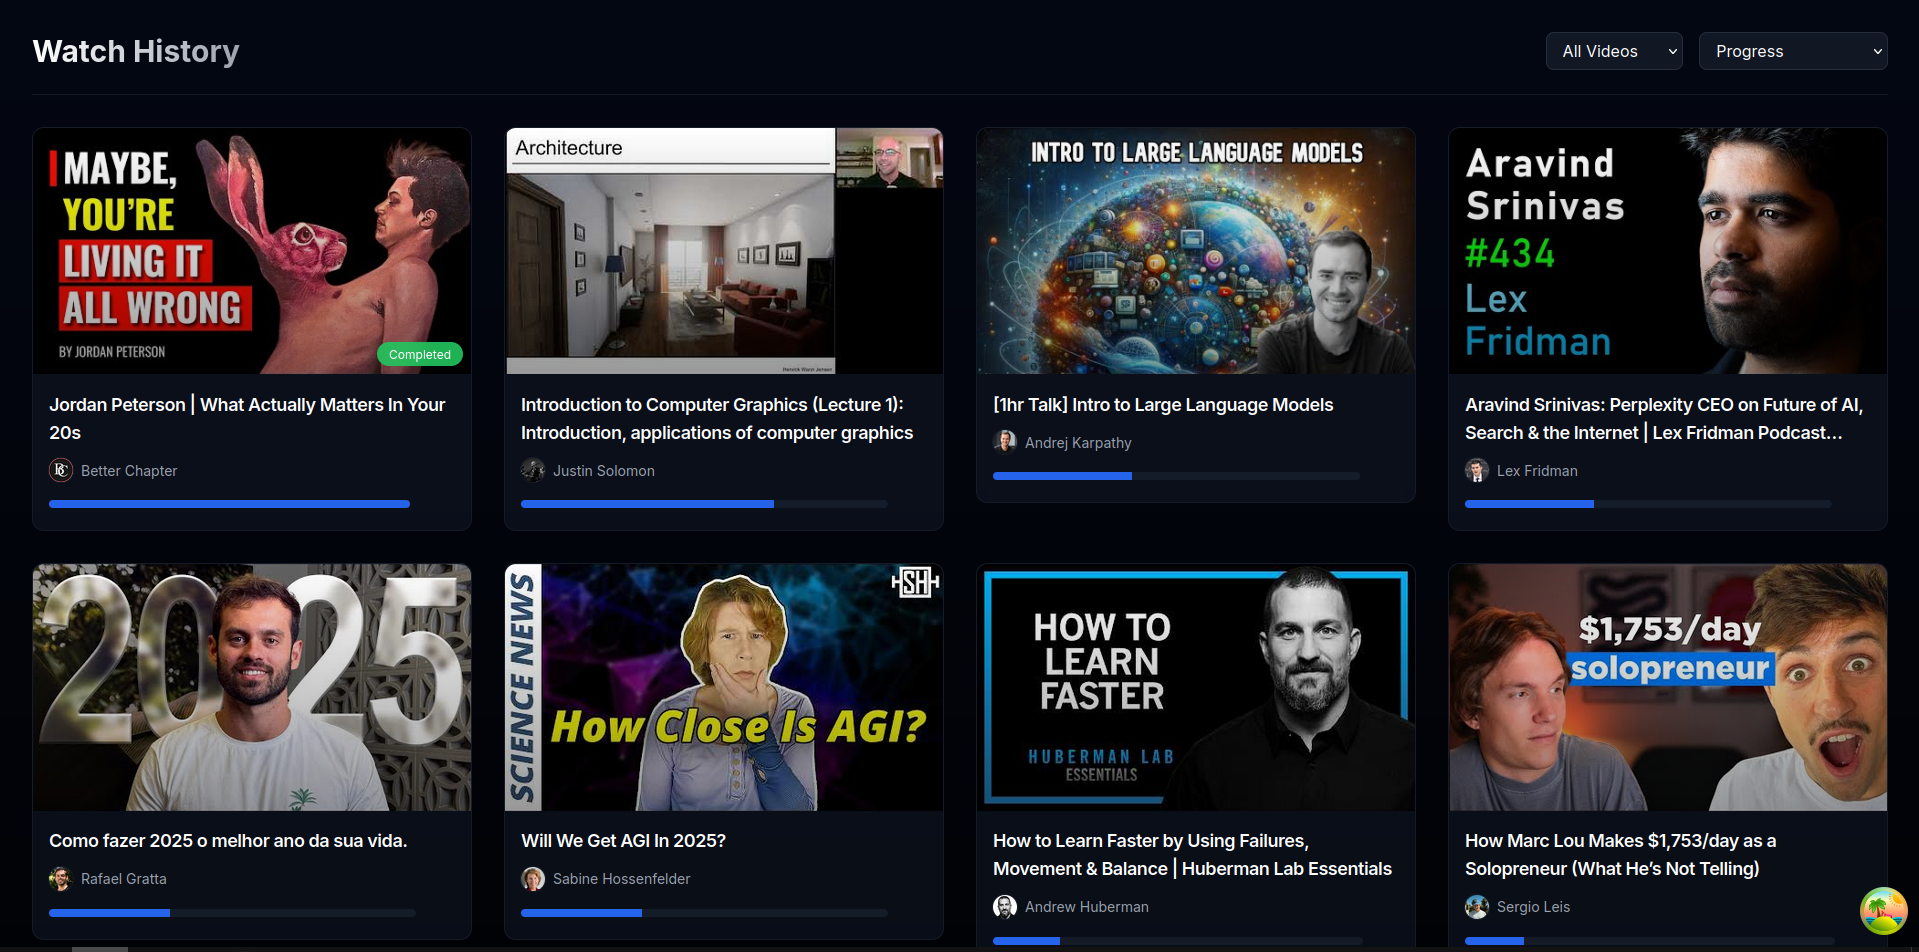
\includegraphics[width=\textwidth,height=0.45\textheight,keepaspectratio]{exemplo-slides/graphics/images/watch history.png}
  \caption{Logs de execução no Beam Serverless GPU demonstrando o tempo de cold start (18s 573ms) na primeira requisição e tempos de resposta reduzidos (aproximadamente 50-100ms) nas requisições subsequentes}
  \label{fig:beam_logs_cold_start}
\end{figure}








A segmentação de texto foi implementada como uma funcionalidade sob demanda, onde o usuário decide quando deseja realizar o processamento. Para cada vídeo, é realizada uma verificação automática para determinar se já existe uma versão segmentada da transcrição armazenada no banco de dados. Caso a versão segmentada já exista, ela é automaticamente carregada e o dropdown exibe "Read Text" como opção selecionada. Caso contrário, o dropdown mostra "Normal Subtitle" e o usuário pode acionar o processo de segmentação selecionando a opção "Read Text".


Durante o processamento, uma requisão para o servidor em beam serverless GPU é realizada e em paralelo um toast notification é exibido para manter o usuário informado sobre o progresso da operação. Ao término do processo, o sistema exibe uma notificação de sucesso ou, em caso de falha, uma mensagem de erro apropriada.

Após o recebimento do texto segmentado, ocorre então um processo de pós processamento, para que nesse texto segmentado, seja reeinserido as informações sobre o tempo que foram perdidas no processo anterior.


\begin{figure}[H]
  \centering
  \begin{subfigure}{\textwidth}
      \centering
      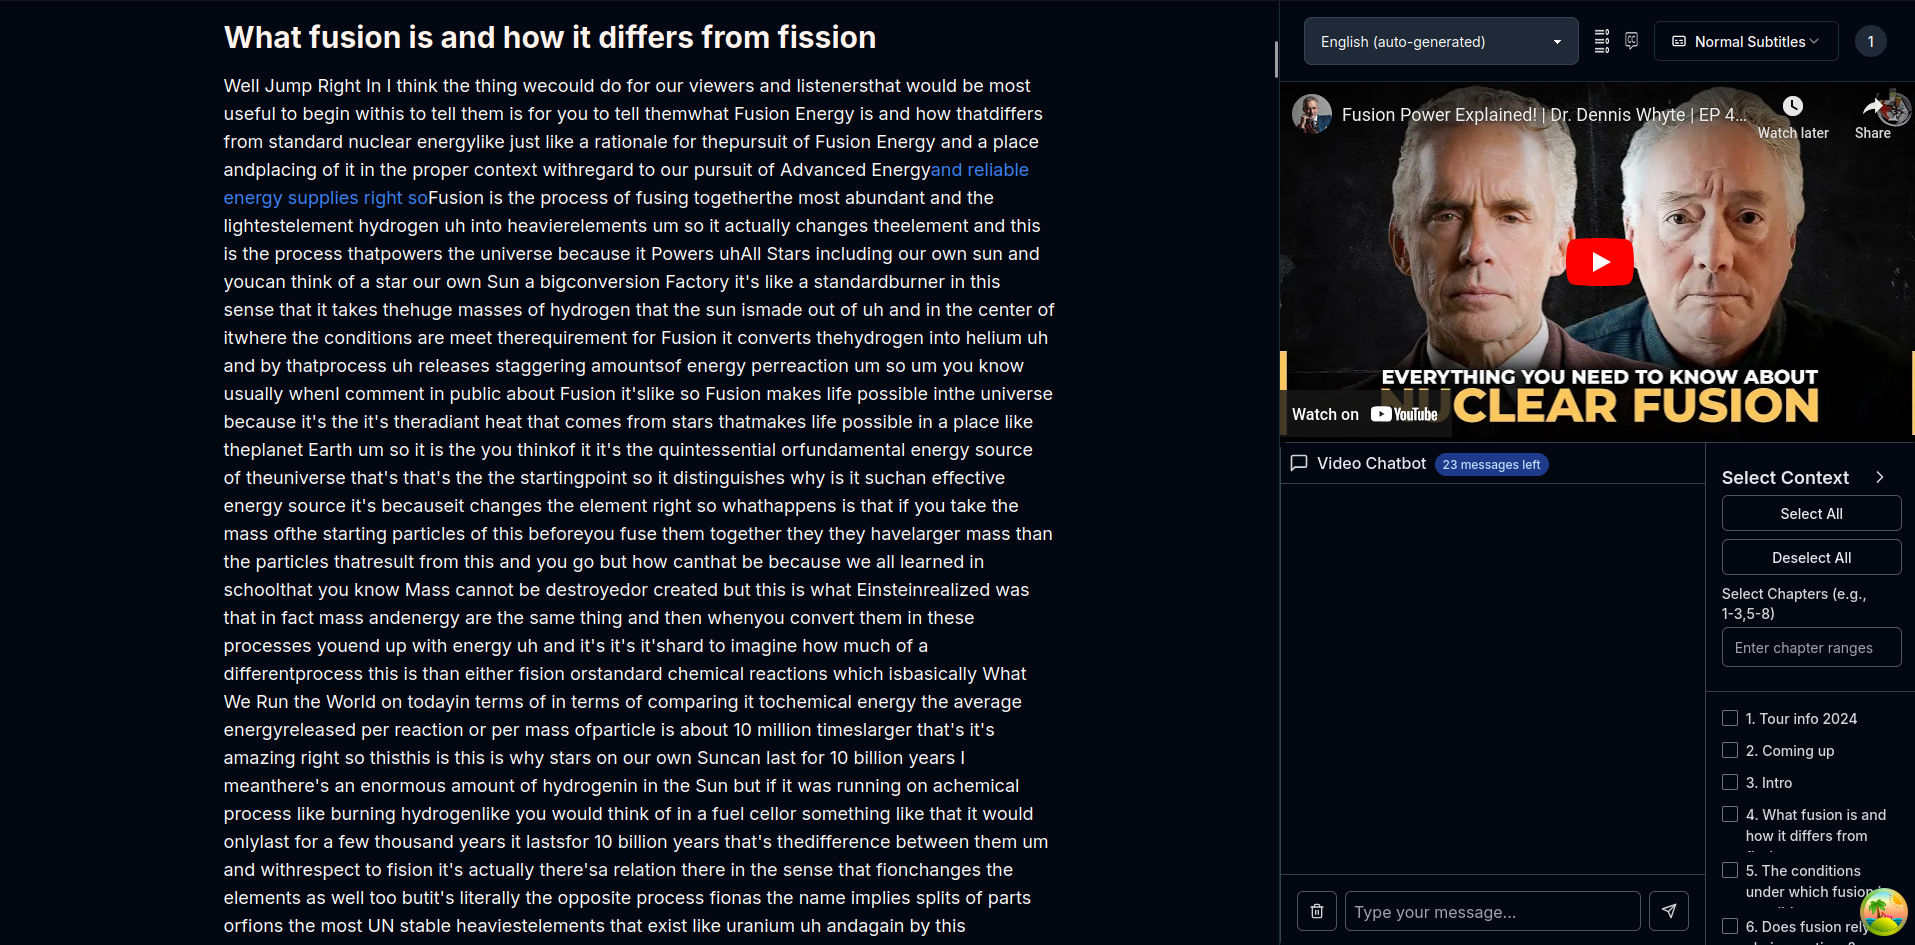
\includegraphics[width=\textwidth,height=0.45\textheight,keepaspectratio]{exemplo-slides/graphics/images/pre-improved-readability.png}
      \caption{Transcrição antes da segmentação}
      \label{fig:pre-improved-readability}
  \end{subfigure}
  
  \begin{subfigure}{\textwidth}
      \centering
      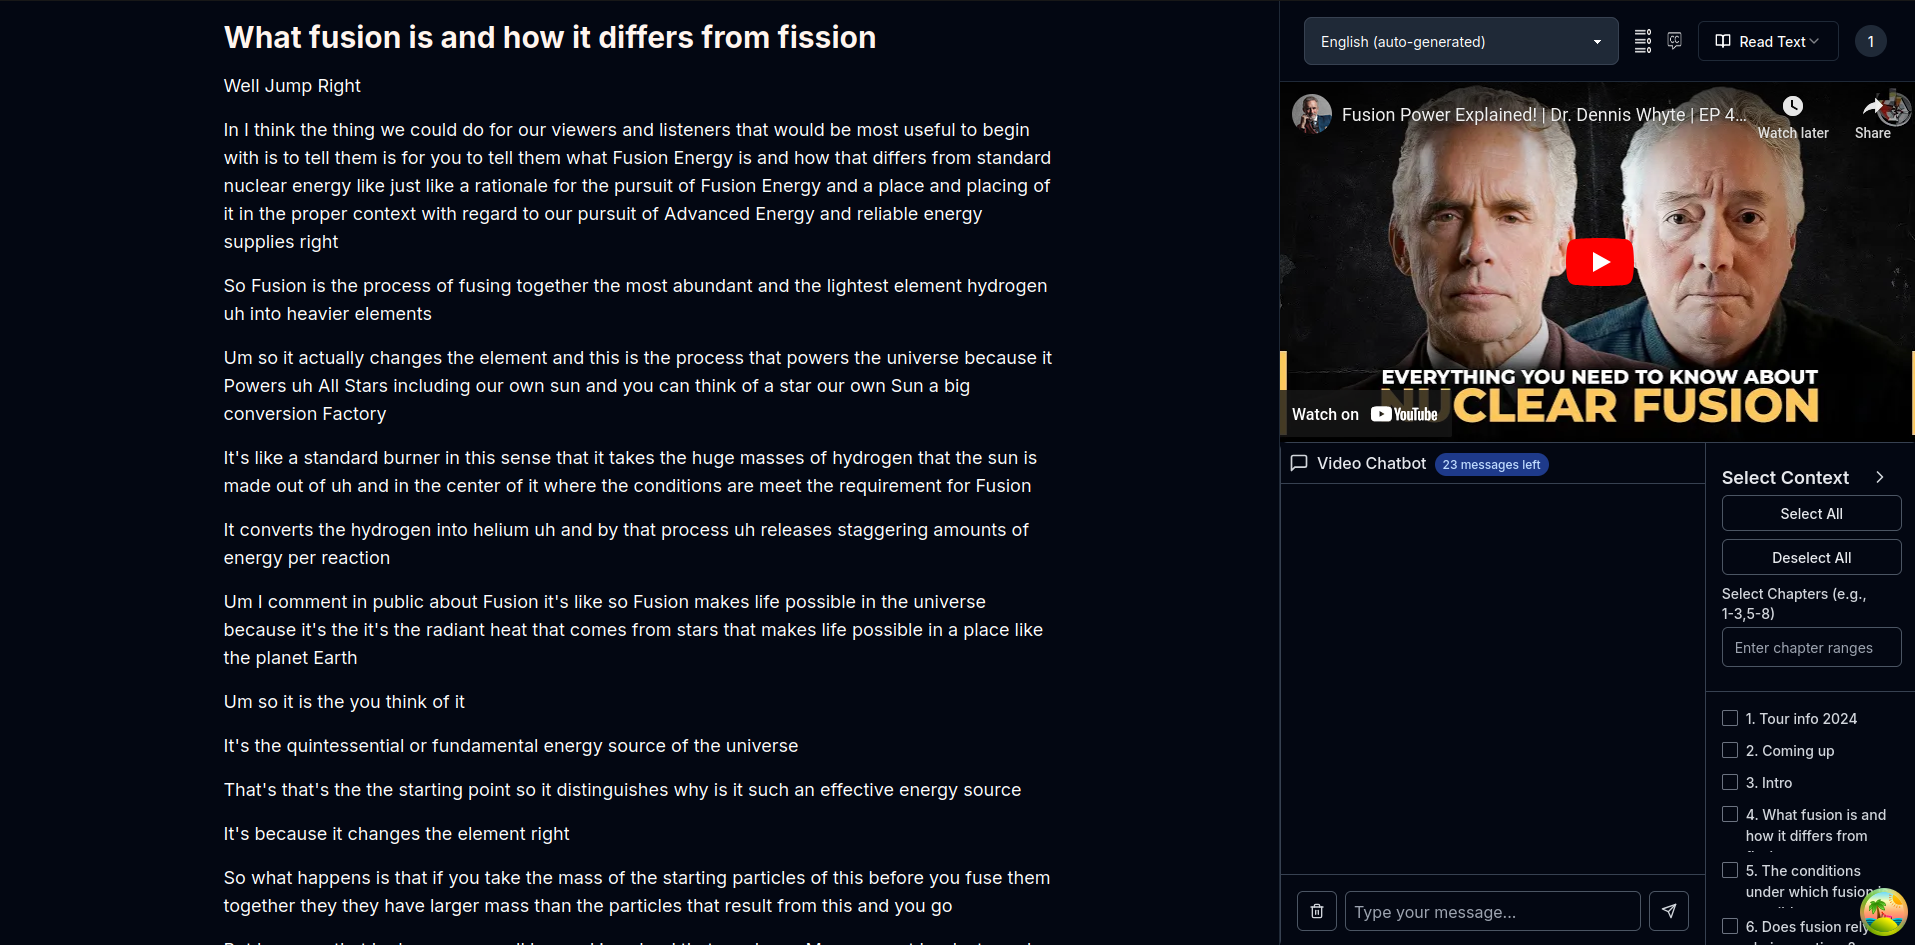
\includegraphics[width=\textwidth,height=0.45\textheight,keepaspectratio]{exemplo-slides/graphics/images/after-improved-readability.png}
      \caption{Transcrição após segmentação com \textit{sat-3l-sm}}
      \label{fig:after-improved-readability}
  \end{subfigure}
  \caption{Comparação antes e após a segmentação de parágrafos.}
  \label{fig:readability-comparison}
\end{figure}






\subsection{Desafios de Implantação em Produção}

A implantação de modelos de machine learning que requerem GPU apresenta desafios significativos, principalmente relacionados a custos e infraestrutura. Apesar do modelo utilizado ser relativamente pequeno, ocupando apenas alguns gigabytes, sua execução utilizando somente CPU é impraticável para uma boa experiência dos usuários, tornando o uso de GPU indispensável. No entanto, manter um servidor dedicado com GPU seria financeiramente inviável para este projeto, dado que servidores assim são bem custosos.

Como alternativa, optou-se por utilizar o Beam Serverless GPU, um serviço que permite o pagamento apenas pelo tempo efetivo de uso do recurso. Esta abordagem oferece uma solução mais econômica, especialmente para cargas de trabalho intermitentes como é o caso do uso nessa aplicação.

No entanto, uma das principais limitações de arquiteturas serverless é o chamado \textit{cold start} - o tempo necessário para inicializar os containers quando não há instâncias ativas. Para mitigar este problema, o Beam Serverless GPU oferece otimizações como a persistência do modelo em disco, eliminando a necessidade de download do modelo a cada inicialização do container.

Em testes realizados em ambiente de produção, observou-se que o primeiro processamento após um cold start levava aproximadamente 17 segundos para completar a inicialização e segmentação do texto. Contudo, as requisições subsequentes eram processadas quase instantaneamente, pois aproveitavam o container já inicializado.


\begin{figure}[H]
  \centering
  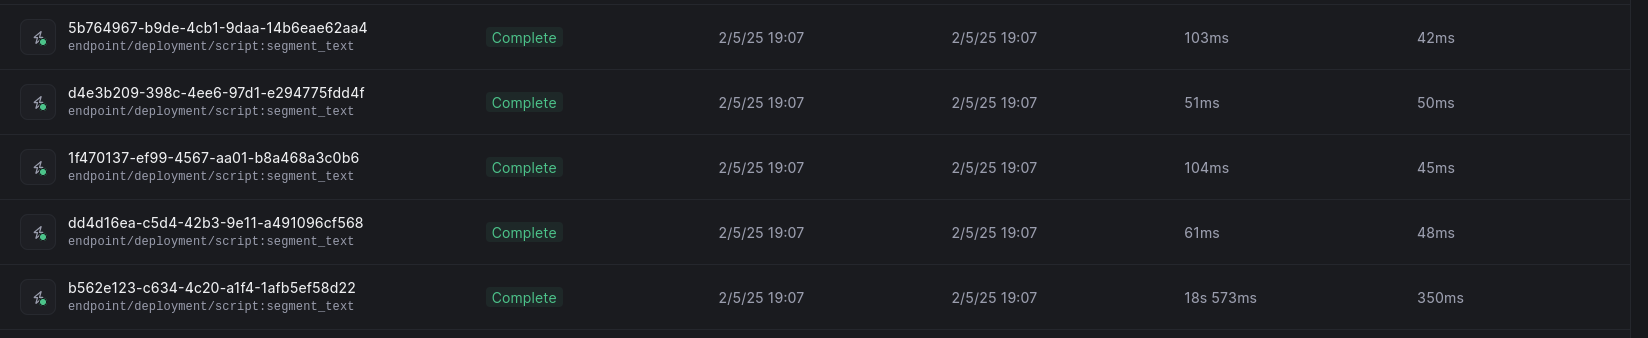
\includegraphics[width=\textwidth,height=0.45\textheight,keepaspectratio]{exemplo-slides/graphics/images/logs-beam.png}
  \caption{Logs de execução no Beam Serverless GPU demonstrando o tempo de cold start (18s 573ms) na primeira requisição e tempos de resposta reduzidos (aproximadamente 50-100ms) nas requisições subsequentes}
  \label{fig:beam_logs_execution}
\end{figure}



ADICIONAR AQUI INFORMAÇÃO DE TEMPO---> o qto demora pra segmentar um texto de X horas






\section{Geração de Capítulos}

A geração automática de capítulos em vídeos do YouTube é um processo essencial para melhorar a navegabilidade e compreensão do conteúdo. A divisão em blocos menores de conteúdo é fundamental para o processo de aprendizagem, pois permite que o estudante absorva o material em partes gerenciáveis, facilitando a retenção e o entendimento.

Além disso, a estruturação em capítulos é crucial para diversas funcionalidades da aplicação:

\begin{itemize}
    \item Permite que usuários selecionem capítulos específicos para discussão no bate-papo com vídeo
    \item Possibilita a geração de quizzes personalizados para cada segmento do conteúdo
    \item Facilita a navegação através da tabela de conteúdo
    \item Viabiliza o rastreamento preciso do progresso do usuário através do histórico de visualização
\end{itemize}

Para implementar esta funcionalidade, a implementação foi baseada na segmentação do texto em parágrafos e na identificação de mudanças de tópico através de um modelo de linguagem de grande escala (LLM).

\subsection{Algoritmo e Implementa\c{c}\~{a}o}

O algoritmo segue um fluxo de processamento em tr\^{e}s etapas principais:

1. \textbf{Estrutura\c{c}\~{a}o do texto:} O conte\'udo transcrito do v\'{i}deo \'{e} segmentado em par\'{a}grafos coerentes, respeitando pausas naturais e mudan\c{c}as de contexto no discurso. Essa segmenta\c{c}\~{a}o melhora a compreens\~{a}o e a an\'{a}lise subsequente do texto.

2. \textbf{Numera\c{c}\~{a}o dos par\'{a}grafos:} Cada par\'{a}grafo recebe um identificador num\'erico no in\'{i}cio, o que permite um referenciamento direto na etapa seguinte.

3. \textbf{Identifica\c{c}\~{a}o de mudan\c{c}as de t\'opico:} Utilizamos um LLM para analisar o texto e determinar os par\'{a}grafos que marcam a transi\c{c}\~{a}o entre t\'opicos distintos. O modelo retorna a lista de n\'{u}meros dos par\'{a}grafos que representam pontos de mudan\c{c}a relevantes no conte\'udo.

\subsection{Integra\c{c}\~{a}o com LLMs}

Para a identifica\c{c}\~{a}o das transi\c{c}\~{o}es de t\'opico, utilizamos function calling para interagir com o LLM. Essa abordagem permite enviar a transcri\c{c}\~{a}o segmentada e numerada, solicitando ao modelo que indique os pontos de mudan\c{c}a mais relevantes. A fun\c{c}\~{a}o chamada retorna uma lista de par\'{a}grafos que representam as mudan\c{c}as de t\'opico, possibilitando a gera\c{c}\~{a}o autom\'atica de cap\'{i}tulos estruturados.

Previamente, foi tentado um m\'etodo em que a function calling solicitava apenas o nome dos t\'opicos de transi\c{c}\~{a}o e seu tempo correspondente. No entanto, observou-se um aumento significativo nas alucina\c{c}\~{o}es do modelo. Ao utilizar a numera\c{c}\~{a}o dos par\'{a}grafos, conseguimos reduzir esse problema, pois conhecendo a posi\c{c}\~{a}o do par\'{a}grafo na transcri\c{c}\~{a}o, podemos determinar com maior precis\~{a}o a sua posi\c{c}\~{a}o temporal no v\'{i}deo.

Essa abordagem garante uma segmenta\c{c}\~{a}o eficiente e adapt\'avel, permitindo uma melhor compreens\~{a}o do conte\'udo dos v\'{i}deos e melhorando a experi\^{e}ncia do usu\'ario ao consumir informa\c{c}\~{o}es em formato de v\'{i}deo.



\begin{figure}[H]
  \centering
  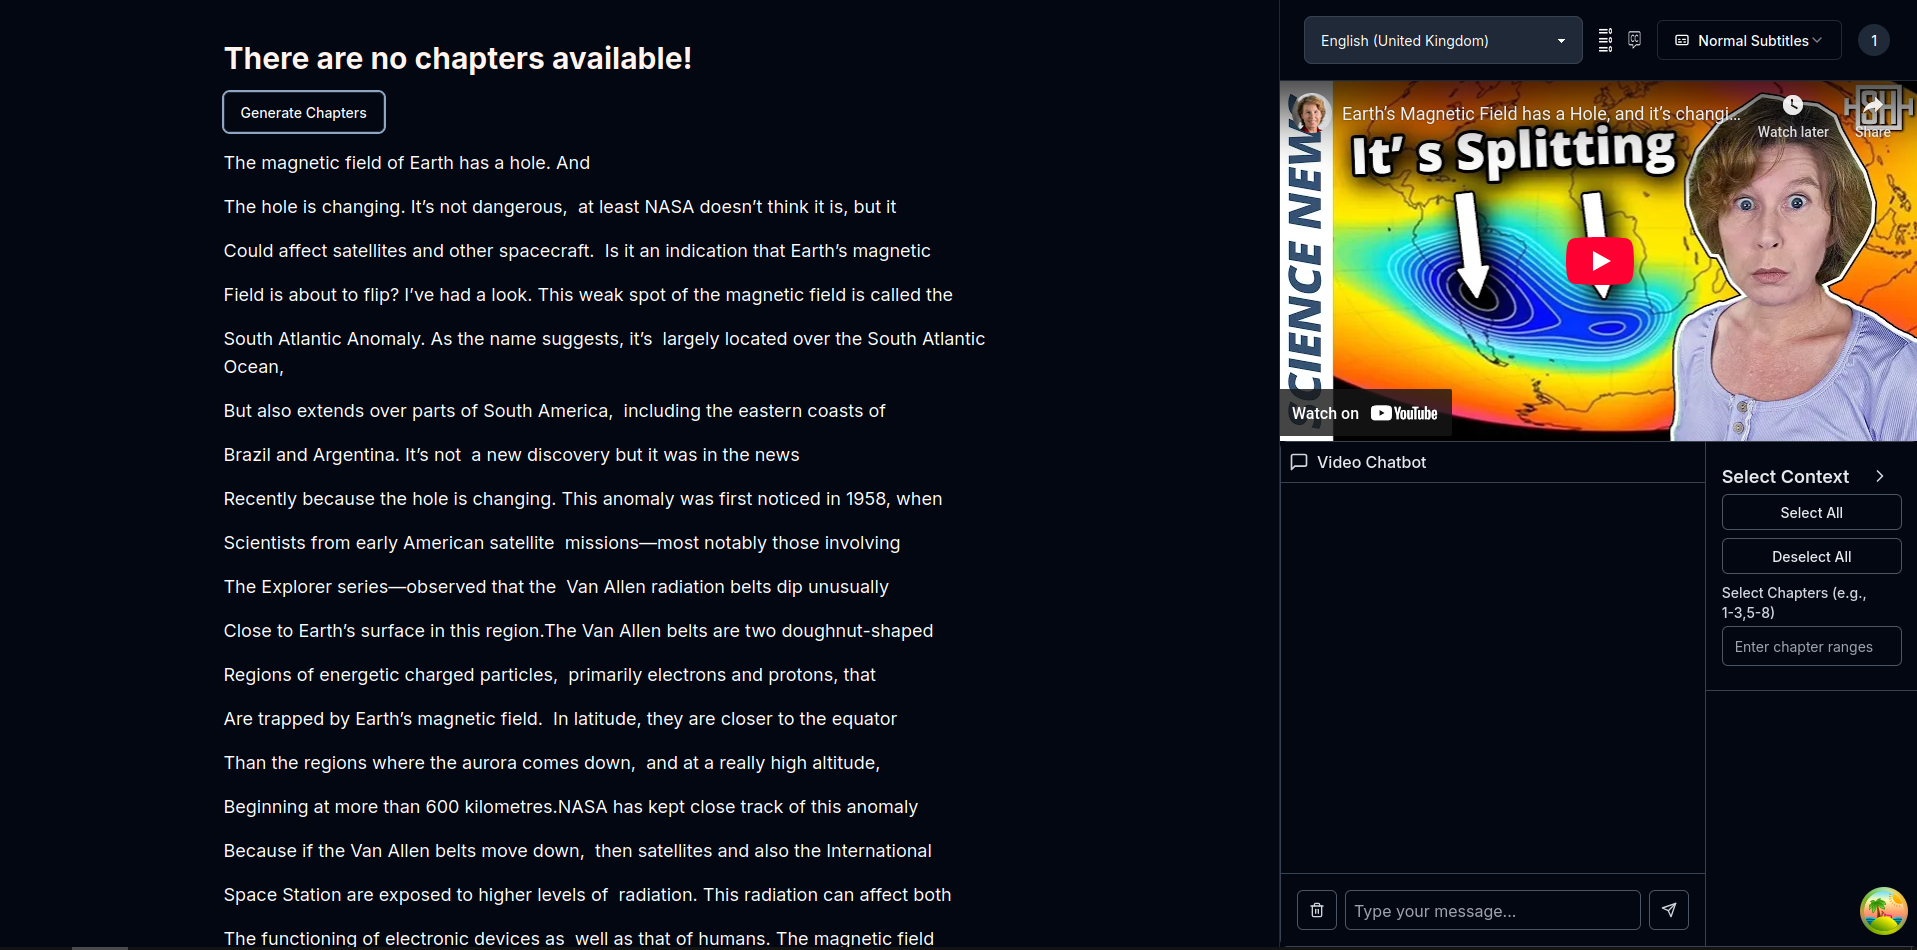
\includegraphics[width=\textwidth,height=0.45\textheight,keepaspectratio]{exemplo-slides/graphics/images/generate-chapters.png}
  \caption{Antes da geração de capítulos. Aviso de que vídeo não possui capítulos e botão para geração}
  \label{fig:generate_chapters_before}
\end{figure}


\begin{figure}[H]
  \centering
  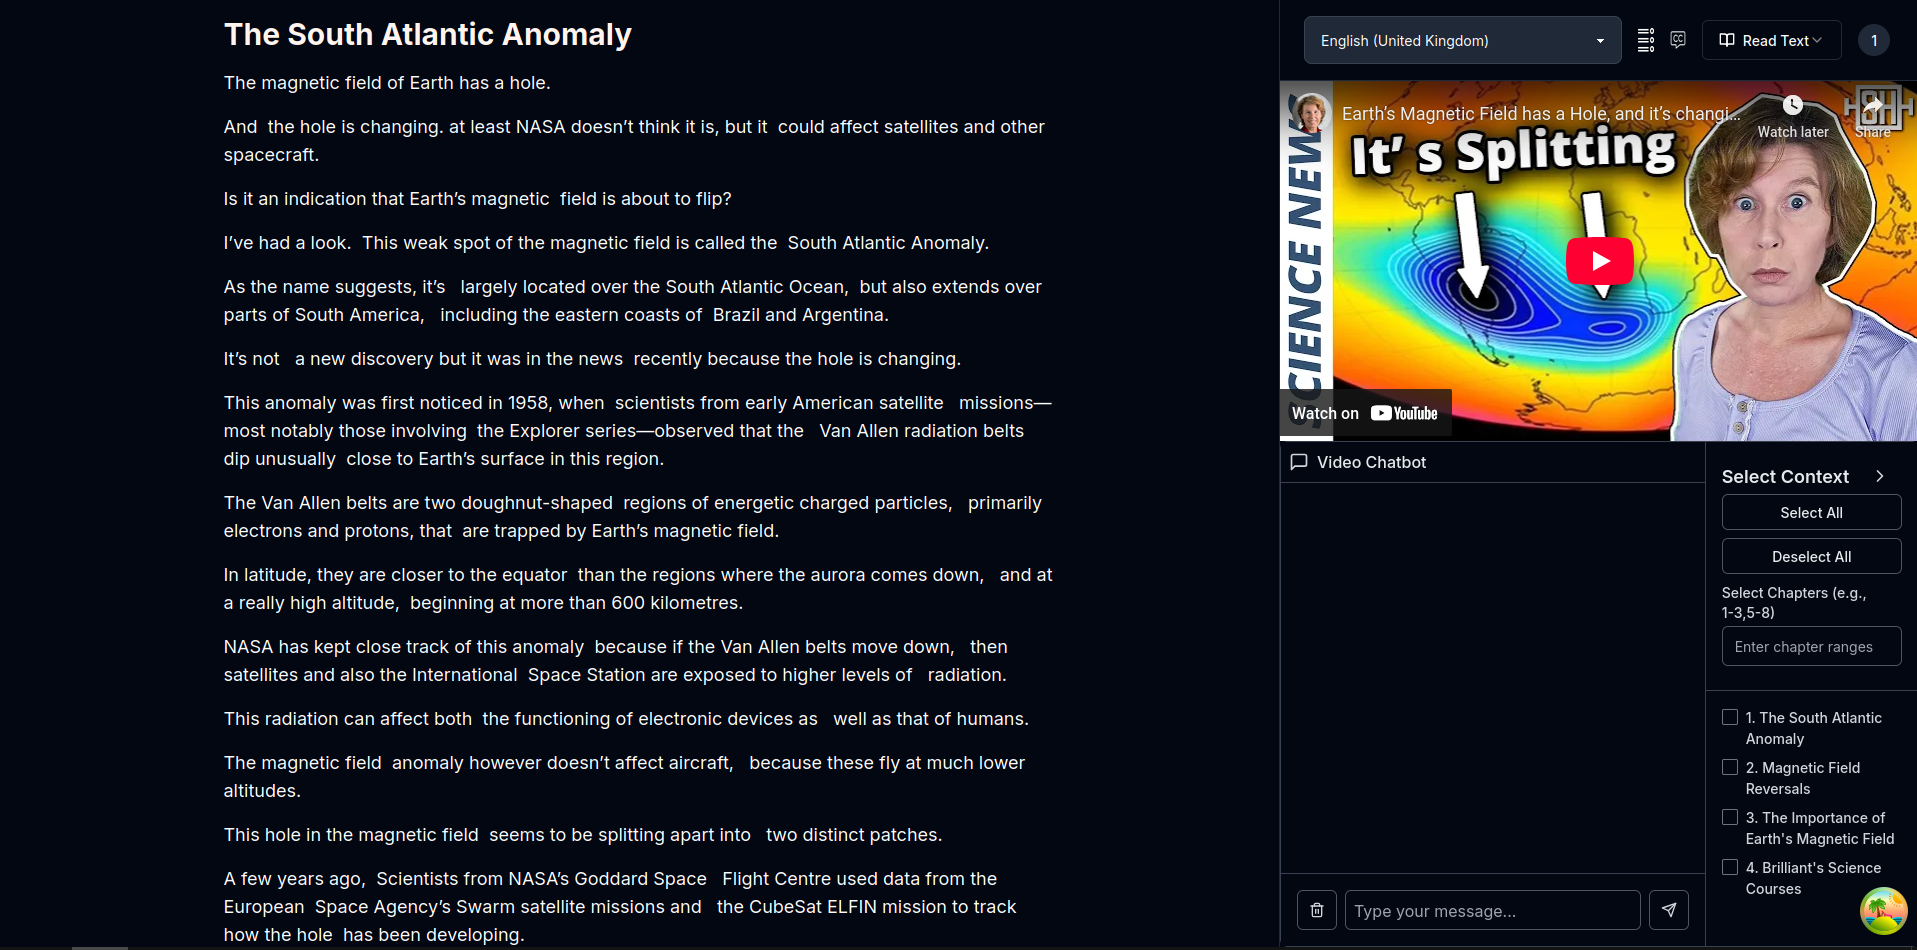
\includegraphics[width=\textwidth,height=0.45\textheight,keepaspectratio]{exemplo-slides/graphics/images/after-chapter-generation.png}
  \caption{Após geração de capítulos.}
  \label{fig:generate_chapters_after}
\end{figure}






\subsection{Tabela de Conteúdos}


\begin{figure}[H]
  \centering
  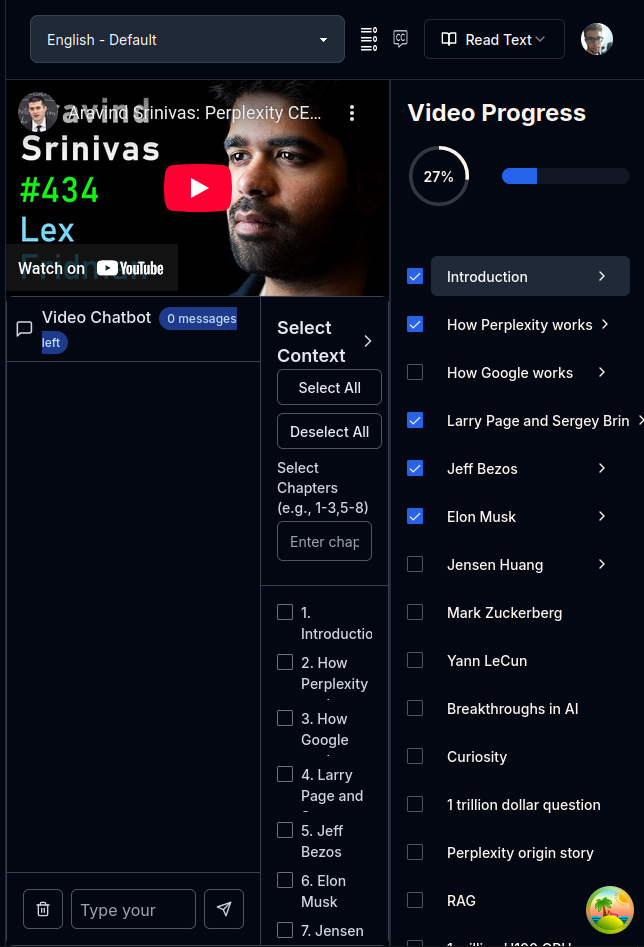
\includegraphics[width=\textwidth,height=0.45\textheight,keepaspectratio]{exemplo-slides/graphics/images/table of contents.png}
  \caption{Tabela de conteúdos gerada automaticamente a partir dos capítulos identificados}
  \label{fig:table_of_contents}
\end{figure}




\subsection{Últimos Vídeos Vistos}

\begin{figure}[H]
  \centering
  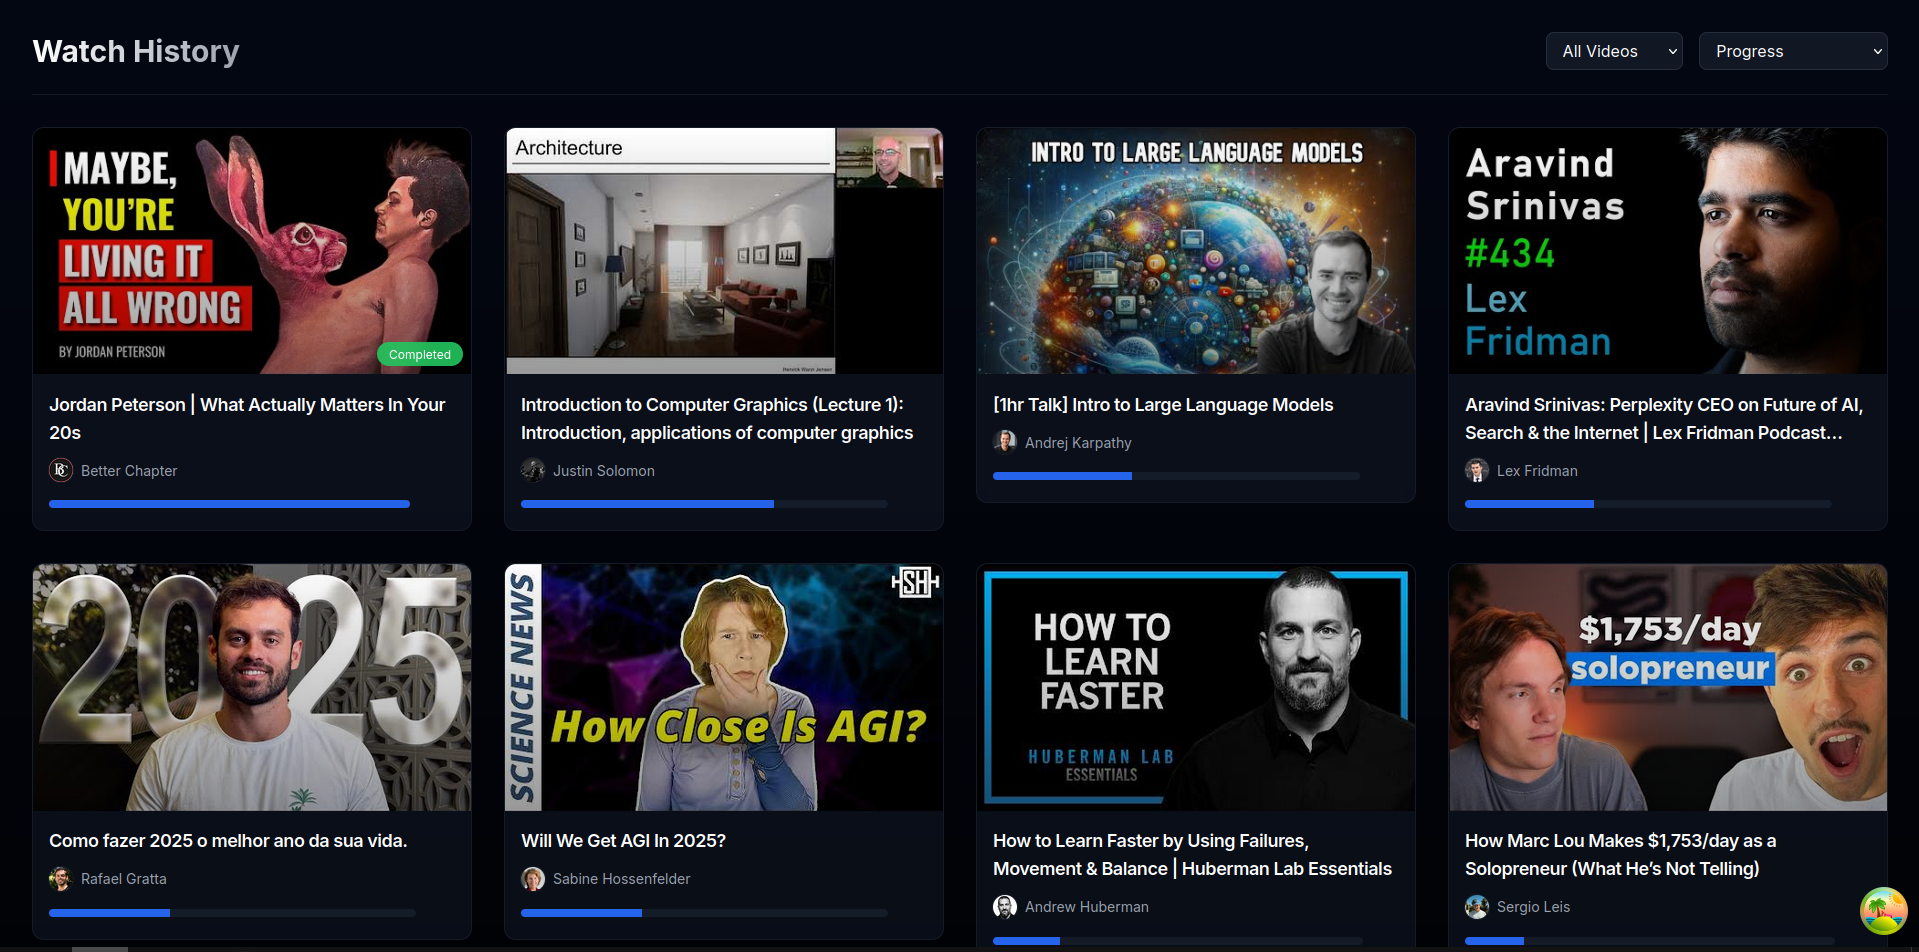
\includegraphics[width=\textwidth,height=0.45\textheight,keepaspectratio]{exemplo-slides/graphics/images/watch history.png}
  \caption{Histórico de visualização mostrando os últimos vídeos assistidos pelo usuário}
  \label{fig:watch_history}
\end{figure}




\section{Transcrição}

A transcrição precisa de vídeos do YouTube é essencial para gerar textos mais confiáveis do que as legendas automáticas, que apresentam qualidade inferior especialmente para línguas diferentes do inglês.

\subsection{Primeira implementação com Whisper}

No fluxo original utilizando o Whisper, o processo consistia em:

1. \textbf{Download otimizado do áudio}:
   - Download apenas da stream de áudio via \texttt{pytubefix}, sem baixar o vídeo
   - Seleção da segunda pior qualidade de áudio, equilibrando precisão e velocidade
   - Progresso do download transmitido em tempo real do backend para o frontend via SSE

2. \textbf{Pré-processamento específico para Whisper}:
   - Divisão do áudio em segmentos de 10 minutos
   - Cortes preferencialmente em momentos de silêncio
   - Envio paralelo dos segmentos para transcrição
   - Necessidade decorrente das limitações do Whisper com arquivos longos
   - Sem feedback de progresso durante a transcrição

\subsection{Migração para o Deepgram}

Com a adoção do Deepgram, o fluxo foi otimizado:

1. \textbf{Download otimizado do áudio mantido}:
   - Mesmo processo de download apenas do áudio via \texttt{pytubefix}
   - Mantida a seleção da segunda pior qualidade para eficiência
   - Feedback em tempo real do progresso via SSE
   - Eliminação da etapa de divisão do áudio

2. \textbf{Transcrição direta}:
   - Envio do arquivo de áudio completo
   - Processamento único sem necessidade de paralelização
   - Estimativa de tempo restante baseada na métrica de 29.8 segundos por hora de áudio do modelo nova-2
   - Capacidade nativa de lidar com longas durações

\subsection{Vantagens adicionais do Deepgram}

O Deepgram oferece recursos avançados ainda não implementados:

\begin{itemize}
  \item Marcação temporal no nível da palavra (word-level timestamps)
  \item Diarização: identificação e segmentação de diferentes interlocutores
    \begin{itemize}
    \item Possibilita diferenciação visual por cores no texto
    \item Permite interações direcionadas no chat com falantes específicos
    \end{itemize}
  \item Programa para startups com crédito inicial de US\$ 200
  \end{itemize}

\subsection{Interface e Experiência do Usuário}

Usuário tem que clicar lá naquele botão de legenda, depois vai pra esse modal, e depois entao apertando no OK, aparece um widget que primeiro irá mostrar o progresso do download e depois irá mostrar uma esmitimativa de tempo pra transcrição.

Finalmente o transcript é adicionado em language selector a o texto é atualizado.


\begin{figure}[H]
  \centering
  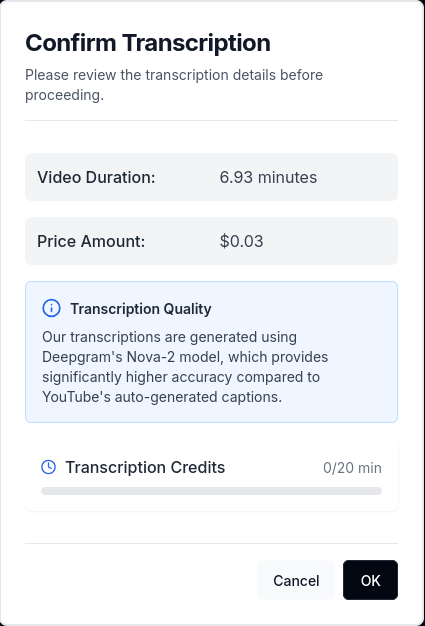
\includegraphics[width=\textwidth,height=0.45\textheight,keepaspectratio]{exemplo-slides/graphics/images/transcription-modal.png}
  \caption{}
  \label{fig:Transcription Modal}
\end{figure}



\section{Gera\c{c}\~ao de Quizzes}

A gera\c{c}\~ao de quizzes para cada cap\'{i}tulo \'e uma funcionalidade essencial, pois permite ao usu\'ario verificar sua compreens\~ao do conte\'udo antes de avan\c{c}ar para a pr\'oxima se\c{c}\~ao. Essa abordagem auxilia na reten\c{c}\~ao do conhecimento, garantindo que os conceitos fundamentais tenham sido absorvidos de maneira eficaz.

Foram desenvolvidas duas interfaces gr\'aficas distintas para os quizzes, adaptadas a diferentes tipos de perguntas:

\begin{itemize}
  \item Interface para quest~oes de \textit{Verdadeiro ou Falso}.
  \item Interface para quest\~oes do tipo \textit{Pergunta e Resposta} (\textit{Q\&A}).

  \end{itemize}

Em ambos os casos, a intera\c{c}\~ao com o quiz \'e feita de maneira din\^amica, utilizando o Vercel AI SDK. A interface do usu\'ario \'e atualizada em tempo real conforme a \textit{Large Language Model} (LLM) gera as respostas. Esse fluxo interativo melhora a experi\^encia do usu\'ario, proporcionando uma sensa\c{c}\~ao de engajamento e imers\~ao no processo de aprendizado.

Para viabilizar essa funcionalidade, utilizamos \textit{function calling}, um mecanismo que permite especificar um \textit{schema} que a LLM deve obedecer ao processar os pedidos. Esse conceito foi previamente abordado na fundamenta\c{c}\~{a}o te\'orica, mas, de maneira resumida, ele garante que as respostas sigam um formato estruturado, permitindo maior controle sobre a sa\'ida gerada pela IA.

Al\'em disso, para ambos os tipos de quiz, o usu\'ario tem a op\c{c}\~ao de personalizar o comportamento da LLM por meio da edi\c{c}\~ao do \textit{prompt} espec\'ifico. Essa personaliza\c{c}\~ao pode ser feita ao clicar no bot\~ao de tr\^es pontos dentro da interface do quiz, permitindo que o usu\'ario defina diretrizes mais precisas para a gera\c{c}\~ao das quest\~oes. Esse recurso adiciona flexibilidade e adapta\c{c}\~ao ao sistema, tornando-o mais vers\'atil para diferentes necessidades e prefer\^encias de aprendizado.

\subsection{Questões discursivas}

\begin{figure}[H]
\centering
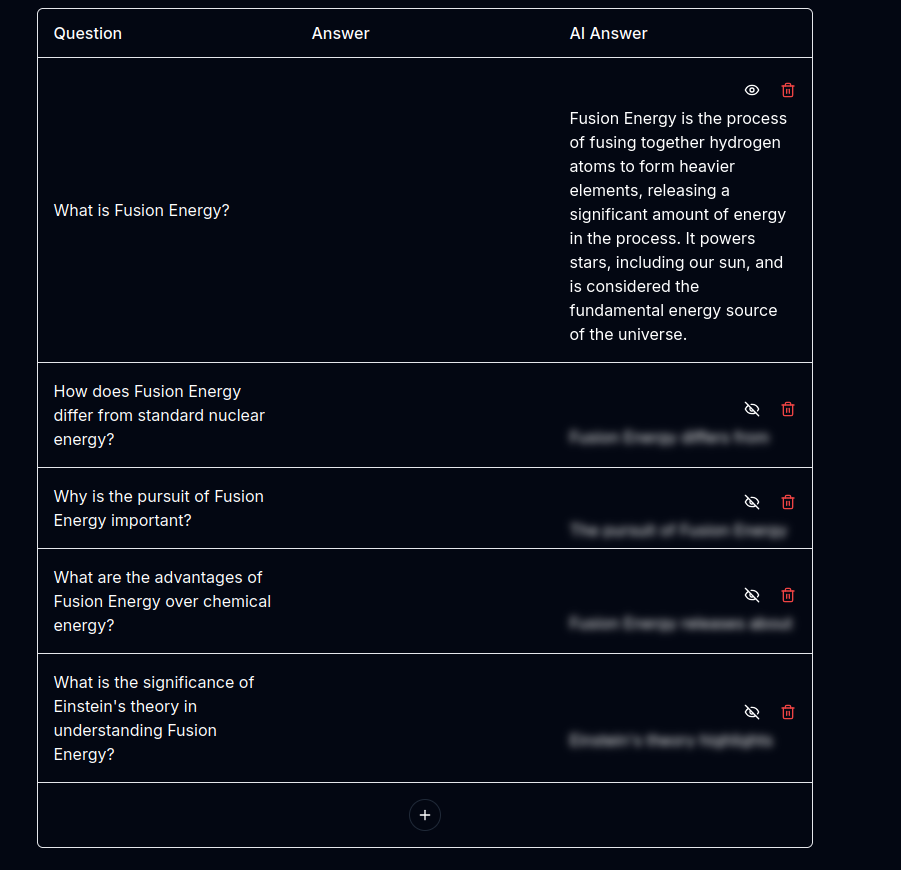
\includegraphics[width=\textwidth,height=0.45\textheight,keepaspectratio]{exemplo-slides/graphics/images/q_a.png}
\caption{Exemplo de interface para perguntas e respostas.}
\label{fig:qa_interface}
\end{figure}

A interface de perguntas e respostas (Q\&A) apresenta uma tabela com três colunas: a primeira exibe a pergunta gerada, a segunda, chamada ``Resposta'', permite ao usuário inserir sua resposta manualmente, e a terceira, ``AI Answer'', que é inicialmente oculta por um efeito de \textit{blur}. A visibilidade dessa coluna pode ser alternada através de um botão, permitindo que o usuário visualize ou oculte a resposta gerada pela IA. O objetivo desse design é incentivar o usuário a tentar responder antes de consultar a resposta fornecida pela IA, promovendo um aprendizado mais ativo e eficaz.


\subsection{Questões de Verdadeiro ou Falso}

\begin{figure}[H]
\centering
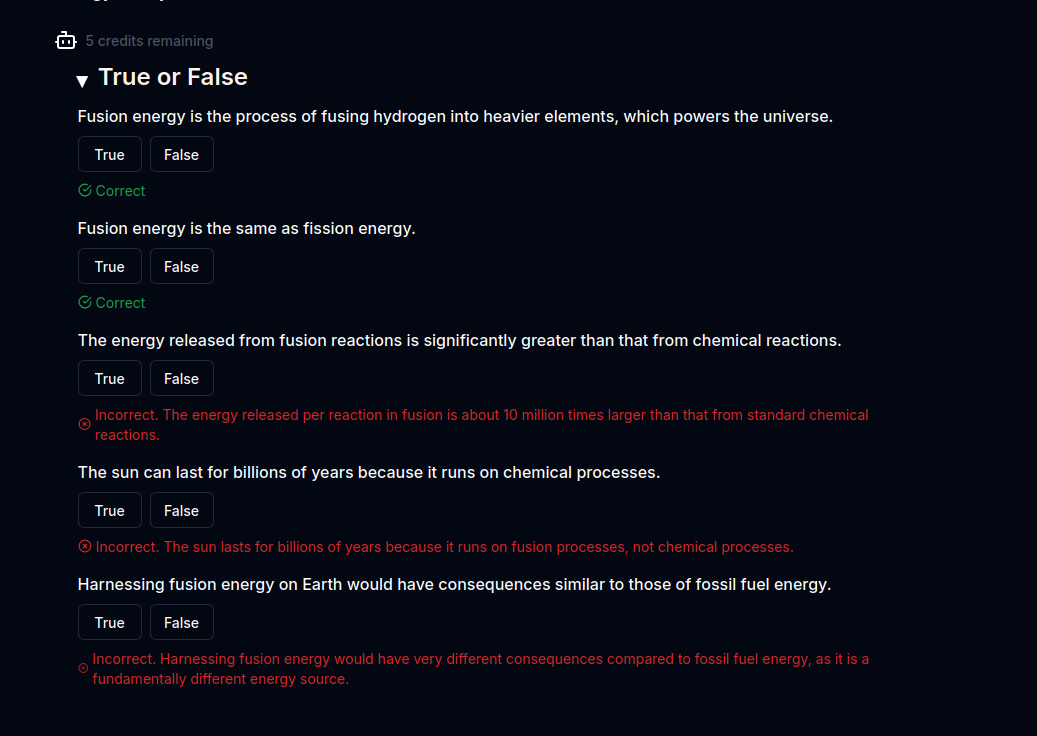
\includegraphics[width=\textwidth,height=0.45\textheight,keepaspectratio]{exemplo-slides/graphics/images/true_or_false.png}
\caption{Exemplo de interface para quest~oes de verdadeiro ou falso.}
\label{fig:true_false_interface}
\end{figure}

Na interface de Verdadeiro ou Falso, as perguntas são apresentadas como afirmações textuais, e abaixo de cada uma há dois botões que permitem ao usuário marcar a resposta como verdadeira ou falsa. Após a seleção um texto adicional surge abaixo, indicando o resultado da resposta: caso esteja correta, a confirmação aparece em verde; caso esteja errada, um texto em vermelho explica o motivo do erro. Esse feedback imediato auxilia na compreensão dos conceitos e melhora a fixação do aprendizado.




\section{Prompt por capítulo}


\section{Bate-Papo com Vídeo}

\subsection{Visão Geral}
O componente de bate-papo com vídeo foi desenvolvido como uma ferramenta interativa que permite aos usuários fazer perguntas e obter respostas contextualizadas sobre o conteúdo de vídeos. O sistema fundamenta-se na análise de legendas e capítulos para fornecer respostas precisas e relevantes, mantendo um gerenciamento eficiente de tokens para otimizar a interação com o modelo de linguagem.

\subsection{Interface do Usuário}
A interface foi projetada com foco na usabilidade e eficiência. No centro da tela, encontra-se o player de vídeo integrado, acompanhado por um painel expansível para seleção de contexto. Abaixo, localiza-se o campo de chat para interação e o histórico da conversa. Um elemento crucial da interface é o botão de exclusão de mensagens, que permite ao usuário limpar todo o histórico de conversa e o contexto selecionado, possibilitando um novo início de interação.

O sistema de seleção de contexto foi implementado de forma flexível, oferecendo duas modalidades principais: seleção através de checkboxes individuais e entrada textual com sintaxe simplificada (por exemplo, "1-3,5" para selecionar os capítulos 1, 2, 3 e 5).

\subsection{Gerenciamento de Contexto e Tokens}
O sistema opera sob parâmetros específicos de controle: um limite de 12.000 tokens para mensagens do sistema e máximo de 120.000 tokens para a conversa completa. Para manter a eficiência, o sistema preserva apenas os cinco pares mais recentes de mensagens ativas.

Para vídeos extensos sem capítulos, um sistema de proteção automática entra em ação. O usuário é notificado através de um aviso sobre o truncamento da legenda, recebendo sugestões para a geração de capítulos. Quando o contexto selecionado excede os limites estabelecidos, o sistema realiza ajustes automáticos, comunicando as alterações através de notificações toast.

\subsection{Implementação Técnica}
\subsubsection{Streaming e Processamento}
O núcleo da implementação utiliza o Vercel AI SDK, responsável pelo gerenciamento de streams de dados em tempo real, processamento de respostas incrementais e manipulação do estado da conexão. Esta escolha tecnológica permite uma experiência fluida e responsiva durante a interação com o vídeo.

\subsubsection{Perspectivas de Evolução}
O sistema foi arquitetado prevendo futuras expansões, com especial atenção para a implementação de um sistema agêntico de seleção de contexto, integração com RAG (Retrieval-Augmented Generation), processamento de diarização e análise semântica avançada.

\subsection{Benefícios e Características}
A implementação atual se destaca pela precisão nas respostas, alcançada através de uma contextualização eficiente. O sistema mantém a coerência conversacional mesmo em diálogos extensos, sem comprometer a qualidade das interações. A interface responsiva e adaptável, combinada com o gerenciamento inteligente de recursos, proporciona uma experiência robusta para análise e discussão de conteúdo em vídeo.

O equilíbrio entre funcionalidade, eficiência e experiência do usuário resulta em uma ferramenta versátil e eficaz para a exploração de conteúdo audiovisual através de conversação natural. A persistência do contexto inicial, combinada com o gerenciamento dinâmico das mensagens, garante respostas consistentes e relevantes ao longo de toda a interação.



\section{Desafios e Soluções}
\subsection{Obtenção dos dados do youtube}
\subsection{Utilização de GPU's em produção}





\chapter{CONCLUSÃO}

O desenvolvimento do VideoLearnAI demonstrou o potencial significativo da integração entre modelos de linguagem natural e tecnologias web modernas para criar experiências educacionais mais efetivas. A plataforma conseguiu transformar o consumo passivo de vídeos em um processo de aprendizagem ativa, oferecendo ferramentas que promovem maior engajamento e compreensão do conteúdo.

\section{Objetivos Alcançados}

Os objetivos inicialmente propostos foram alcançados através da implementação bem-sucedida das cinco funcionalidades principais:

\begin{enumerate}
    \item \textbf{Melhoria da Legibilidade das Legendas:} A implementação do modelo SAT (Segment Any Text) proporcionou uma solução eficiente e precisa para a segmentação de texto, superando as limitações encontradas na abordagem inicial com LLMs. Esta funcionalidade demonstrou ser fundamental para melhorar a experiência de leitura e compreensão do conteúdo.

    \item \textbf{Geração de Capítulos:} O sistema de geração automática de capítulos, combinando segmentação de texto com análise por LLMs, mostrou-se eficaz na organização estruturada do conteúdo, facilitando a navegação e o acesso a informações específicas.

    \item \textbf{Legendas de maior qualidade:} A geração de legendas com o serviço Deepgram ao invés das legendas geradas automaticamente pelo youtube, resultou em um processo mais eficiente e preciso de transcrição, com benefícios adicionais como marcação temporal no nível da palavra e capacidade de diarização dos locutores.

    \item \textbf{Quizzes Interativos:} Superando as limitações do consumo passivo de vídeo, os questionários interativos com feedback em tempo real promovem engajamento ativo através de exercícios práticos e reflexivos, maximizando a absorção do conteúdo.

    \item \textbf{Bate-Papo Contextual:} O sistema de chat contextualizado proporcionou uma forma natural e eficiente de interação com o conteúdo do vídeo, com gerenciamento adequado de contexto, transparente para o usuário.
\end{enumerate}

\section{Trabalhos Futuros}

O desenvolvimento do VideoLearnAI abriu diversas possibilidades para aprimoramentos e expansões futuras:

\subsection{Diarização e Análise de Múltiplos Falantes}

\begin{itemize}
  \item Aprimorar o texto da transcrição utilizando a diarização do Deepgram através de elementos visuais distintivos (legendas coloridas, avatares, badges) para cada interlocutor
  \item Integrar a identificação de falantes às demais funcionalidades, enriquecendo o contexto no chat, quizzes.
\end{itemize}


\subsection{Otimizações Técnicas}
\begin{itemize}
    \item Implementação de RAG (Retrieval-Augmented Generation) para:
        \begin{itemize}
            \item Melhorar a precisão das respostas no chat
            \item Possibilitar análises avançadas de debates, incluindo fact-checking, qualidade argumentativa e identificação de falácias
            \item Integração com diarização para análise específica por interlocutor
        \end{itemize}
    \item Redução adicional dos tempos de cold start em funções serverless
    \item Aprimoramento do sistema de cache para conteúdos frequentemente acessados
\end{itemize}

\subsection{Expansão de Funcionalidades}
\begin{itemize}
    \item Sistema de repetição espaçada utilizando os quizzes gerados
    \item Elementos de gamificação:
        \begin{itemize}
            \item Sistema de ranking por vídeo
            \item Métricas de engajamento e aprendizado
            \item Recompensas por participação ativa
        \end{itemize}
    \item Suporte a mais formatos de conteúdo além do YouTube
    \item Ferramentas colaborativas para estudo em grupo
    \item Sistema de exportação de notas e resumos
    \item Integração com plataformas de ensino existentes
\end{itemize}

\subsection{Melhorias na Experiência do Usuário}
\begin{itemize}
    \item Interface adaptativa para diferentes dispositivos e contextos de uso
    \item Mais opções de personalização visual
    \item Suporte expandido para múltiplos idiomas
\end{itemize}

A aplicação desenvolvida nesse trabalho demonstrou a viabilidade de combinar tecnologias avançadas de IA com princípios de aprendizagem ativa. Embora em fase inicial, a aplicação apresenta potencial significativo para transformar como as pessoas aprendem através de conteúdo audiovisual educativo.




% Bibliografia http://liinwww.ira.uka.de/bibliography/index.html um
% site que cataloga no formato bibtex a bibliografia em computacao
% \bibliography{nomedoarquivo.bib} (sem extensao)
% \bibliographystyle{formato.bst} (sem extensao)

\bibliographystyle{abnt}
\bibliography{bibliografia} 

% Apêndices (Opcional) - Material produzido pelo autor
\apendices
\chapter{Um Apêndice}

% Anexos (Opcional) - Material produzido por outro
\anexos
\chapter{Um Anexo}

Bla blabla blablabla bla.  Bla blabla blablabla bla.  Bla blabla
blablabla bla.  Bla blabla blablabla bla.  Bla blabla blablabla bla.
Bla blabla blablabla bla.  Bla blabla blablabla bla.  Bla blabla
blablabla bla.  Bla blabla blablabla bla.  Bla blabla blablabla bla.
Bla blabla blablabla bla.  Bla blabla blablabla bla.  Bla blabla
blablabla bla.  Bla blabla blablabla bla.  Bla blabla blablabla bla.
Bla blabla blablabla bla.  Bla blabla blablabla bla.  Bla blabla
blablabla bla.  Bla blabla blablabla bla.  Bla blabla blablabla bla.
Bla blabla blablabla bla.

Bla blabla blablabla bla.  Bla blabla blablabla bla.  Bla blabla
blablabla bla.  Bla blabla blablabla bla.  Bla blabla blablabla bla.
Bla blabla blablabla bla.  Bla blabla blablabla bla.  Bla blabla
blablabla bla.  Bla blabla blablabla bla.  Bla blabla blablabla bla.
Bla blabla blablabla bla.  Bla blabla blablabla bla.  Bla blabla
blablabla bla.  Bla blabla blablabla bla.  Bla blabla blablabla bla.
Bla blabla blablabla bla.  Bla blabla blablabla bla.  Bla blabla
blablabla bla.  Bla blabla blablabla bla.  Bla blabla blablabla bla.
Bla blabla blablabla bla.




\end{document}

